% ======== 卷首下（9行20字）========
\chapter*{欽定儀象考成卷首下}
\begin{正文}
\end{正文}\clearpage
\thispagestyle{empty}\noindent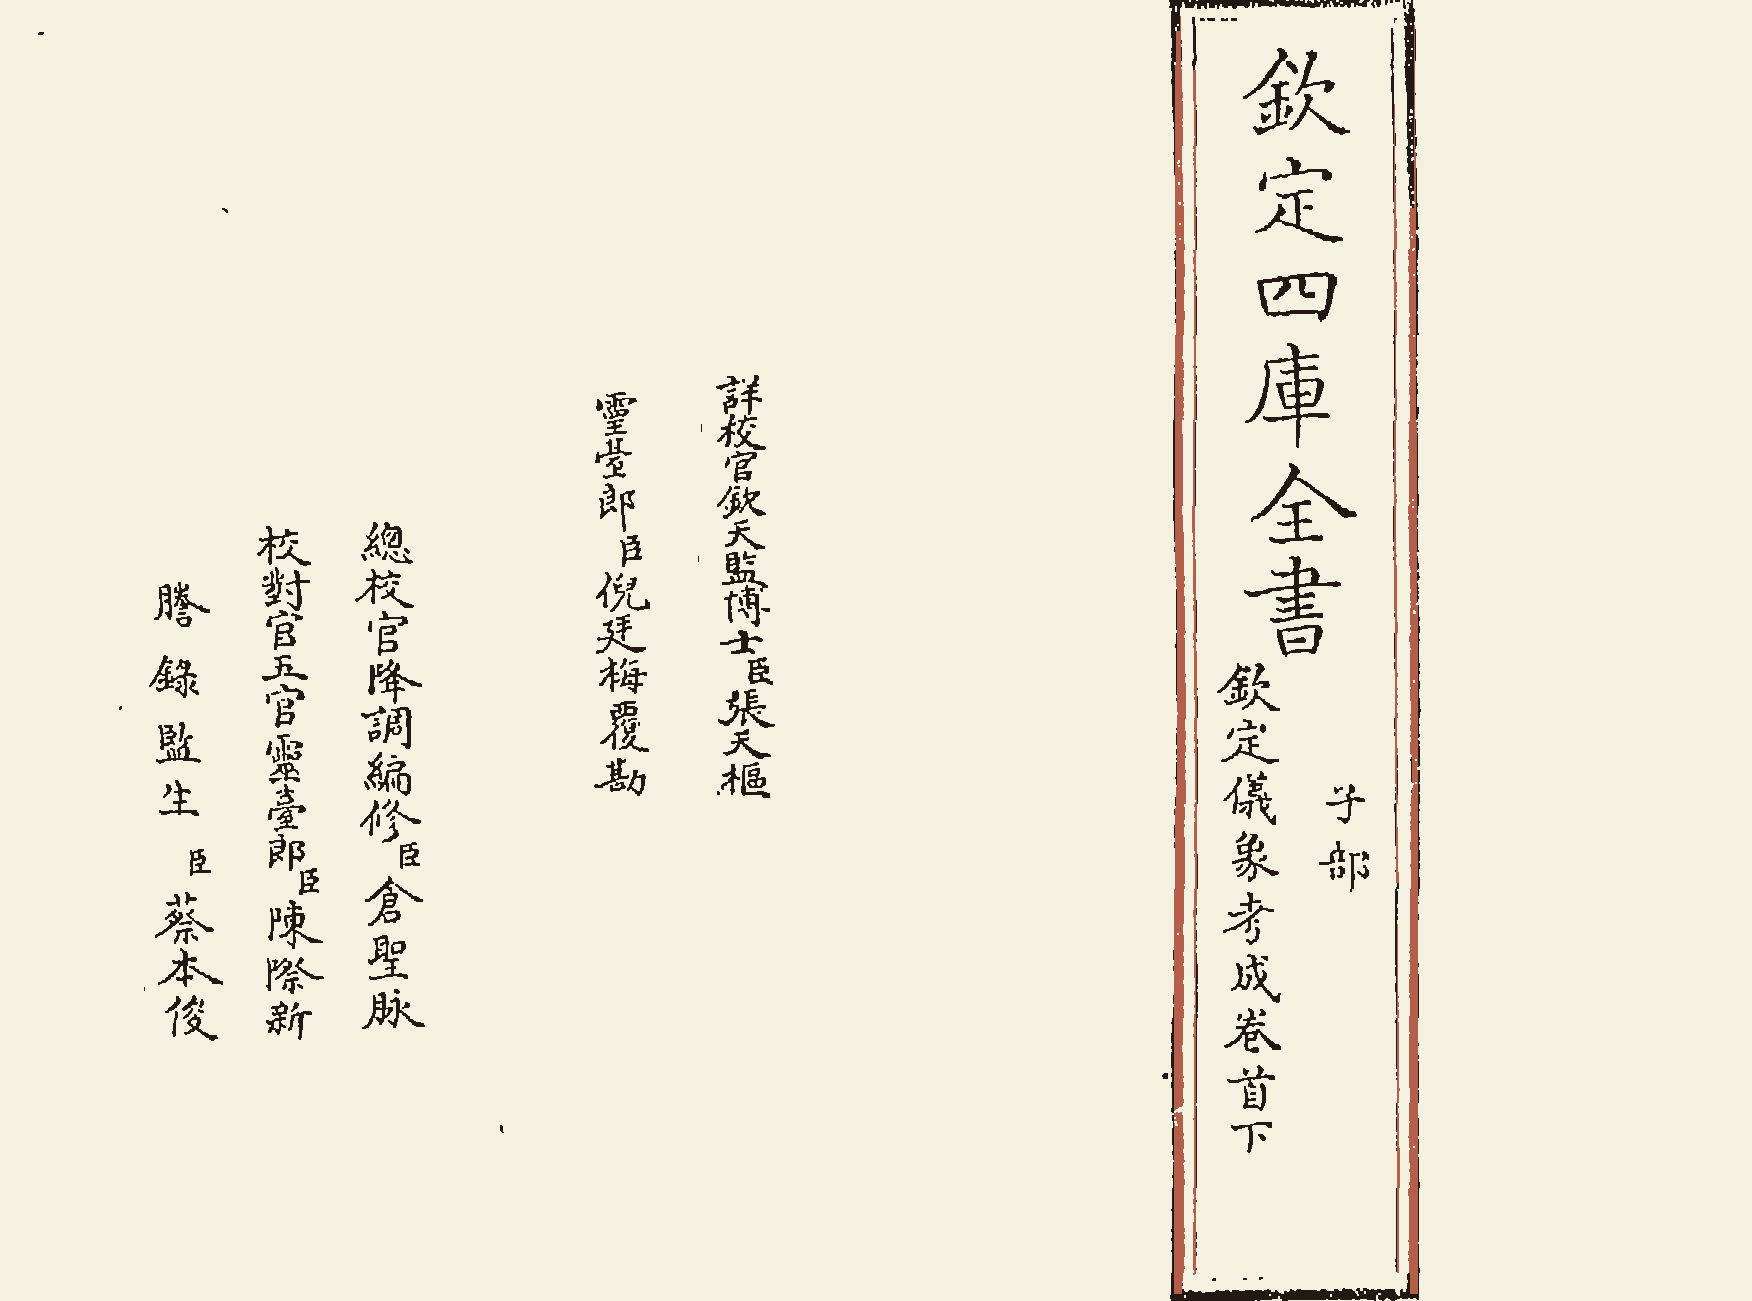
\includegraphics[width=\paperwidth,height=\paperheight,keepaspectratio]{img/0232.png}\clearpage
\begin{正文}
% ---- 册793 葉233 ----
\SetPageNumber{1}
欽定四庫全書\换行
欽定儀象考成卷首下\换行
御製璣衡撫辰儀説卷下\换行
　　用法\换行
　　算法\换行
\char"200B\relax\换行
\char"200B\relax\换行
\char"200B\relax\换行
\char"200B\relax\换行
\char"200B\relax\换行
\char"200B\relax\换行
\char"200B\relax\换行
\char"200B\relax\换行
\char"200B\relax\换行
\char"200B\relax\换行
\char"200B\relax
\par
% ---- 册793 葉236 ----
御製璣衡撫辰儀説卷下之一\换行
　用法\换行
　　測太陽時刻\换行
　　測日出入時刻及晝夜永短\换行
　　測太陽赤道緯度\换行
　　測午正太陽髙弧\换行
　　測太陽赤道經度\换行
　　測月星赤道經緯度\换行
　　測恒星求時刻\换行
　　測月五星求時刻\换行
　　測月星當中及偏度\换行
　　測月星出入地平時刻\换行
　　測南北真線\换行
　　測北極髙度\换行
　　測黄赤距度\换行
　　測黄白距度
\par
% ---- 册793 葉237 ----
　　測太陽時刻\换行
法以四遊圏東西推轉窺衡南北低昂令太陽從衡孔\换行
透光圓正或用薫黒玻璃置於下端衡孔視上端圓孔\换行
十字線正當太陽中心則窺衡與太陽參直乃視四遊\换行
圏下周指時度表臨於天常赤道之某時刻分即太陽\换行
時刻也若二分前後日影為赤道所礙則用窺衡上面\换行
立表測之\双列{\右小列{常時不為赤道所}\左小列{礙亦用此表為便}}若午正及卯酉前後日影\换行
為子午圏及龍柱所礙則用窺衡上面平行立表測之\换行
以四遊窺衡對凖太陽令上端表圓孔十字線影從下\换行
端表圓孔正中透出上端表直線影從下端表直縫正\换行
中透出\双列{\右小列{測時刻止用經度可止取直線影}\左小列{若測緯度則必取圓孔十字線影}}視指時度表\换行
所指即得太陽時刻若指時度表為子午圏所礙則易\换行
用借弧指時度表次用平行立表測定日影視借弧指\换行
時度表所指時刻加一小時即得太陽時刻盖借弧之\换行
長當遊旋赤道之十五度當天常赤道之一小時又借\换行
表在四遊圏之西所指時刻在本時前故加一小時即
\par
% ---- 册793 葉240 ----
為本時刻分也\换行
　　測日出入時刻及晝夜永短\换行
法於太陽出入地平時按前法測得太陽出入時刻乃\换行
計距午正前後若干刻分倍之即得晝刻計距子正前\换行
後若干刻分倍之即得夜刻\换行
　　測太陽赤道緯度\换行
法如前測凖太陽視窺衡下端指緯度表所指四遊圏\换行
右面距赤道度分即得太陽赤道緯度表指赤道北太\换行
陽緯度為在赤道南表指赤道南太陽緯度為在赤道\换行
北盖窺管以圓心為樞上端所窺在赤道北下端所指\换行
必在赤道南上端所窺在赤道南下端所指必在赤道\换行
北也\换行
　　測午正太陽髙弧\换行
法於午正時測得太陽赤道緯度在赤道北與赤道髙\换行
五十度五分相加在赤道南與赤道髙五十度五分相\换行
減即午正太陽髙弧也
\par
% ---- 册793 葉241 ----
　　測太陽赤道經度\换行
法用恒星作距測之取所知近午正前後一恒星\双列{\右小列{午正}\左小列{前後}}\换行
\双列{\右小列{取其𫎇氣少}\左小列{易得確凖也}}以其赤道經度之對衝用綰經度表於遊\换行
旋赤道綰定四遊圏\双列{\右小列{凡以儀器測星其上當星處為星}\左小列{之正位其下當人目處則星之對}}\换行
\双列{\右小列{冲故以星經度之對冲於}\左小列{遊旋赤道綰定四遊圏}}又任設一時用綰時度表於\换行
其時刻之對衝綰定天常赤道\双列{\右小列{天常環面乃日影所照}\左小列{之時其對冲則太陽所}}\换行
\双列{\右小列{臨之正位故於設時之對冲綰之如設丑正初}\左小列{刻則綰於未正初刻即太陽臨於丑正之位也}}乃将四\换行
逰圏帶定遊旋赤道用窺衡測凖距星隨之左旋𠉀至\换行
所設時刻\双列{\右小列{或鐘表或漏}\左小列{壺須得確凖}}視綰時度表對於遊旋赤道之\换行
某宫度分即太陽赤道經度也\双列{\右小列{環面時刻之對冲即太}\左小列{陽所臨之正位故其所}}\换行
\双列{\右小列{對遊旋赤道之宫}\左小列{度即太陽經度}}\换行
又法先以恒星作距測金星次以金星作距測太陽如\换行
金星晨見則於太陽未出之前取在金星西之一恒星\换行
作距以其赤道經度用平行線測經度表於遊旋赤道\换行
安定\双列{\右小列{三測皆係經度若距星之經度用對冲則測得之}\左小列{經度又須加減半周故距星不用對冲所測亦即}}\换行
\双列{\右小列{得本}\左小列{度也}}令一人用此平行線表窺定距星隨之左旋一人
\par
% ---- 册793 葉244 ----
用四遊窺衡測金星兩人同時測定乃視四遊圏指時\换行
度表所指遊旋赤道之宫度分即金星赤道經度次以\换行
金星赤道經度用平行線測經度表於遊旋赤道安定\换行
令一人窺定金星隨之左旋一人於太陽始出時用四\换行
遊窺衡測太陽乃視四遊圏指時度表所指遊旋赤道\换行
之宫度分即得太陽赤道經度若金星夕見則於太陽\换行
将入時任於某宫初度安定平行線測經度表令一人\换行
窺定金星又令一人用四遊窺衡測太陽視太陽距金\换行
星若干度記定俟太陽既入後取金星東之一恒星作\换行
距按前法測得金星赤道經度内減太陽距金星之度\换行
\双列{\右小列{星在東日}\左小列{在西故減}}即得太陽赤道經度也\双列{\右小列{太陽光大惟月及金}\左小列{星可以兩見然月有}}\换行
\双列{\右小列{視差不如用}\左小列{金星為凖也}}\换行
　　測月星赤道經緯度\换行
法於昏後曉前任設一時以本日太陽赤道經度與次\换行
日太陽赤道經度比例得本時太陽赤道經度\双列{\右小列{七政時}\左小列{憲書所}}\换行
\双列{\右小列{列乃子正之度子正後七政皆有行分故以本日子正}\左小列{之度分與次日子正之度分相減餘為一日十二時所}}
\par
% ---- 册793 葉245 ----
\双列{\右小列{行之分與設時距子正之時分為比例得設時距子}\左小列{正之行分加於本日子正之度分得本時之度分}}用\换行
綰時度表於遊旋赤道綰定又以所設時刻之對冲於\换行
天常赤道綰定𠉀至所設時刻用四遊窺衡測月星乃\换行
視指時度表所指遊旋赤道宫度加半周\双列{\右小列{環面時刻之}\左小列{對冲即為太}}\换行
\双列{\右小列{陽之正位環面之宮度却}\左小列{為月星之對冲故加半周}}即得所測月星赤道經度隨\换行
察指緯度表所指四遊圏距赤道南北度分即得所測\换行
月星赤道緯度也\双列{\右小列{緯之南北與前測}\左小列{太陽緯度法同}}\换行
又法用恒星作距測之以距星之赤道經度用平行線\换行
測經度表於遊旋赤道安定令一人用此平行線表窺\换行
定距星隨之左旋一人用四遊窺衡測月星兩人同時\换行
測定乃視指時度表所指遊旋赤道之度分即所測月\换行
星之赤道經度隨察指緯度表所指四遊圏之度分即\换行
得所測月星之赤道緯度也\换行
　　測恒星求時刻\换行
法先以恒星赤道經度用綰經度表於遊旋赤道綰定\换行
四遊圏次約計測時為某時依前法比例得本時太陽
\par
% ---- 册793 葉248 ----
赤道經度\双列{\右小列{太陽每日行一度於時為四分每一時行五}\左小列{分於時為二十秒故約計測量之時比例得}}\换行
\双列{\右小列{其時赤道經度即}\左小列{可用以測時刻也}}用綰時度表綰定遊旋赤道将四遊\换行
圏帶遊旋赤道推轉用窺衡測定恒星乃視綰時度表\换行
對於天常赤道之某時刻分加六時即太陽時刻也\双列{\右小列{天}\左小列{常}}\换行
\双列{\右小列{赤道之時刻乃日影對照之時故}\左小列{加六時始為太陽所臨之時刻也}}\换行
　　測月五星求時刻\换行
法以本時太陽赤道經度用綰時度表綰定遊旋赤道\换行
以月五星本時赤道經度之對冲用綰經度表於遊旋\换行
赤道綰定四遊圏将四遊圏帶遊旋赤道推轉用窺衡\换行
測定月星乃視綰時度表對於天常赤道之某時刻分\换行
加六時即得太陽時刻若太陽近子正前後綰時度表\换行
為子午圏所礙則向東或西借三十度綰定測之視所\换行
對時刻加減一時\双列{\右小列{向東借則加}\左小列{向西借則減}}即得太陽時刻若月五\换行
星近赤道或近午正前後為諸圏所礙則用窺管上面\换行
立表及平行立表測之與前測太陽時刻法同\换行
　　測月星當中及偏度
\par
% ---- 册793 葉249 ----
法以四遊窺衡隨時測月或星視指時度表當天常赤\换行
道之某時刻分記之\双列{\右小列{近午正則易用借弧}\左小列{指時度表加一小時}}午正為當中\换行
無偏度午正前為偏東午正後為偏西乃以距午時分\换行
變赤道度每一時為三十度每一小時為十五度每一\换行
分為十五分每一秒為十五秒共之為所偏度凡推月\换行
星當中及偏度者用此法測之則離合可辨凡有求時\换行
刻者用此法測定則時刻可推也\换行
　　測月星出入地平時刻\换行
法以本日子正月五星赤道經度或恒星經度之對冲\换行
用綰經度表於遊旋赤道綰定四遊圏又以本日子正\换行
太陽經度用綰時度表綰定遊旋赤道爰以四遊窺衡\换行
於月星出入地平時測之視綰時度表當天常赤道之\换行
某時刻分加六時為本日月星出入時刻之通數復計\换行
測時距本日子正後若干時刻比例得太陽行分變時\换行
\双列{\右小列{每一度為四分每十五分}\左小列{為一分每十五秒為一秒}}為太陽時差比例得月五星\换行
行分變時為月五星時差\双列{\右小列{恒星則無行}\左小列{分亦無時差}}乃於前所測月
\par
% ---- 册793 葉252 ----
星出入時刻之通數減太陽時差加月五星時差即得\换行
月星出入地平時刻盖日與月星測時皆用子正經度\换行
而子正後太陽有右旋之行分則時刻必差而早月五\换行
星亦有右旋之行分則時刻必差而遲\双列{\右小列{時刻左旋七政}\左小列{皆右旋太陽有}}\换行
\双列{\右小列{右旋之行分則測時太陽之經度必在所測時刻之前}\左小列{故差而早月五星有右旋之行分則測時月星之方位}}\换行
\双列{\右小列{必在所測時刻}\左小列{之後故差而遲}}故減太陽時差加月五星時差\双列{\右小列{若五星}\左小列{逆行則}}\换行
\双列{\右小列{時差}\左小列{亦減}}方為月星出入地平真時此與前測月星求時刻\换行
法同理設時可以預知故先求本時經度而後測月星\换行
出入難以懸定故先測而後加減時差其理相通其用\换行
尤便也\换行
　　測南北真線\换行
法於太陽出地平時測其距午東赤道度又於太陽入\换行
地平時測其距午西赤道度\双列{\右小列{測得太陽出入地平距午}\左小列{正前後若干時分變赤道}}\换行
\双列{\右小列{度即得距午正}\左小列{東西赤道度}}兩距午度相等則子午圏之向即南北\换行
真線若日出距午東之度多日入距午西之度少則子\换行
午圏之午正偏西若日出距午東之度少日入距午西
\par
% ---- 册793 葉253 ----
之度多則子午圏之午正偏東\双列{\右小列{此言午正乃子}\左小列{午圏之正南}}以兩測\换行
之距午度相減折半即所偏之赤道經度\双列{\右小列{若求地平偏}\左小列{度則用三角}}\换行
\双列{\右小列{法推之見算}\左小列{法第八則}}依所偏之度作線即南北真線也\换行
又法於冬至後測織女第一星昏刻此星當酉正之位\换行
以四遊圏安於酉正測其去極度若干\双列{\右小列{九十度内減赤}\左小列{道緯度餘即去}}\换行
\双列{\右小列{極}\左小列{度}}旦刻此星當卯正之位以四遊圏安於卯正測其去\换行
極度若干\双列{\右小列{織女星在赤道丑宫七度赤道北三十八度}\左小列{半冬至後半月内昏旦可以兩見故専取此}}\换行
\双列{\右小列{星測}\左小列{之}}兩去極度相等則子午圏之向即南北真線若卯\换行
正位測得去極度多酉正位測得去極度少則東逺西\换行
近即子午圈之北極偏西若卯正位測得去極度少酉\换行
正位測得去極度多則東近西逺即子午圈之北極偏\换行
東以兩測之去極度相減折半即所偏之赤道緯度\双列{\右小列{若}\左小列{求}}\换行
\双列{\右小列{地平偏度則用三角法}\左小列{推之見算法第十五則}}依所偏之度作線即南北真線\换行
也盖南北真線自北極過天頂平分赤道之地平上半\换行
周是為午正故向南測者以午正為凖向北測者以北\换行
極為凖太陽隨天左旋其出地入地距午必相等若其
\par
% ---- 册793 葉256 ----
不等必儀之午正偏也恒星繞地左旋其在東在西去\换行
極必相等若其不等必儀之北極偏也依其偏度正之\换行
則南北真線得矣又按渾儀經緯與天同象測太陽亦\换行
可用緯度測恒星亦可用經度然不及右二法之簡明\换行
推測精熟法理自見今不具悉也\换行
　　測北極髙度\换行
法於冬至前後以四遊圏安於正北測天權星\双列{\右小列{即北斗}\左小列{第四星}}\换行
昏刻此星在北極之下測其去極度若干旦刻此星在\换行
北極之上測其去極度若干\双列{\右小列{天權星今在赤道辰宫初}\左小列{度赤道北五十八度冬至}}\换行
\双列{\右小列{前後半月内昏旦可以}\左小列{兩見故専取此星測之}}兩去極度相等則儀之北極髙\换行
度與天合若在上之去極度少在下之去極度多則儀\换行
之北極差髙若在上之去極度多在下之去極度少則\换行
儀之北極差下以兩測之去極度相減折半即所差之\换行
地平緯度於儀之北極髙度加減之\双列{\右小列{差髙則減}\左小列{差下則加}}即天之\换行
北極髙度也盖天之北極無星故取大星之環繞北極\换行
上下者測之星之去極有定度則上下兩測之去極必
\par
% ---- 册793 葉257 ----
等若其不等則儀之髙下差也依其差度加減之則在\换行
天之北極髙度得矣又按舊法用地平緯儀測鉤陳大\换行
星以其在北極上下兩髙度相加折半得北極髙度取\换行
其距地髙無𫎇氣也今用渾儀測之則鉤陳大星為儀\换行
樞所礙須用借弧故取用天權星測其去極之較以備\换行
一例若以所測在北極上之去極度與所設北極髙度\换行
相加以所測在北極下之去極度與所設北極髙度相\换行
減得兩地平髙度相加折半得北極髙度與用鉤陳大\换行
星之理同\换行
　　測黄赤大距\换行
法於冬至日午正初刻測太陽在赤道南若干度分夏\换行
至日午正初刻測太陽在赤道北若干度分若冬至夏\换行
至皆在午正初刻則所測日距赤道南北之緯度即黄\换行
赤大距度若冬至夏至不正當午正則又用前測太陽\换行
赤道經度法測得太陽距冬夏至前後若干度分用有\换行
太陽赤道經緯度求黄赤交角之法\双列{\右小列{見算法}\左小列{第四則}}求得黄赤
\par
% ---- 册793 葉260 ----
交角即黄赤大距度也盖黄道與赤道斜交春秋分時\换行
太陽正當赤道春分後秋分前太陽在赤道北夏至而\换行
極北秋分後春分前太陽在赤道南冬至而極南故致\换行
日者必於冬夏二至今用弧線三角形法測得逐日之\换行
距緯皆可以推大距然春秋分前後黄道斜而緯差大\换行
以推大距其理𨼆而難知冬夏至前後黄道横而緯差\换行
微以推大距其象顯而易見故冬夏致日古今之通義\换行
也\换行
　　測黄白距限\双列{\右小列{距限即大距因大距又有大小故}\左小列{名距限以别之見數象考成後編}}\换行
法於春分日上弦秋分日下弦月距交九十度時測得\换行
月距赤道北若干度分春分日下弦秋分日上弦月距\换行
交九十度時測得月距赤道南若干度分與黄赤大距\换行
相減餘為黄白二道最大之距限又於冬至日望月距\换行
交九十度時測得月距赤道北若干度分夏至日望月\换行
距交九十度時測得月距赤道南若干度分與黄赤大\换行
距相減餘為黄白二道最小之距限盖白道與黄道斜
\par
% ---- 册793 葉261 ----
交月距交九十度則距黄道最逺故測黄白大距必於\换行
月距交九十度時然黄白大距與黄道成直角黄赤大\换行
距與赤道成直角惟冬夏二至黄道經圈與赤道經圈\换行
合為一線故測黄白大距又必於月當冬夏二至時\双列{\右小列{上}\左小列{編}}\换行
\双列{\右小列{専取月當夏至為其距地髙也}\左小列{若以對待而言則兼用冬夏至}}夫月距交九十度而又\换行
當冬夏二至則兩交必在春秋二分當是時而值兩弦\换行
則日必在春秋分而適當兩交值朔望則日必在冬夏\换行
至而距交九十度上編之法謂兩弦時交角大\双列{\右小列{交角之}\左小列{度即大}}\换行
\双列{\右小列{距}\左小列{度}}朔望時交角小後編之法謂日在兩交時交角大日\换行
距交九十度時交角小極二説之異致至此而得其合\换行
故測黄白大距必於春秋分兩弦冬夏至望日\双列{\右小列{朔日不}\左小列{見月故}}\换行
\双列{\右小列{惟用}\左小列{望日}}月距交九十度時測之春分之日上弦秋分之日\换行
下弦而月距交九十度是月當夏至而日在兩交也春\换行
分之日下弦秋分之日上弦而月距交九十度是月當\换行
冬至而日在兩交也以兩弦與日在兩交而論皆交角\换行
大冬至之日望而月距交九十度是月當夏至而日距
\par
% ---- 册793 葉264 ----
交九十度也夏至之日望而月距交九十度是月當冬\换行
至而日距交九十度也以朔望與日距交九十度而論\换行
皆交角小各測其距赤道度與黄赤大距相減則最大\换行
最小之黄白距限皆得矣按月行出黄道南為陽厯為\换行
正交\双列{\右小列{今為}\左小列{中交}}入黄道北為陰厯為中交\双列{\右小列{今為}\左小列{正交}}夏至在陰厯\换行
冬至在陽厯則月距赤道校黄道為逺故於所測距赤\换行
道度内減黄赤大距餘為黄白大距夏至在陽厯冬至\换行
在陰厯則月距赤道校黄道為近故於黄赤大距内減\换行
所測距赤道度餘為黄白大距又按古法黄白大距不\换行
逾六度弦望無殊故曰春秋致月今法交角有大小故\换行
又必兼於冬夏至測之也\换行
又法推得月離黄道冬夏至時預於前數刻或以太陽\换行
作距用綰時度表綰定時刻或以恒星作距用平行線\换行
測經度表對定距星皆以四遊圏指時度表對冬夏至\换行
宫度安定候月行至二至線上乃以窺衡測月距赤道\换行
南北緯度若干與黄赤大距相減餘為月距黄道南北
\par
% ---- 册793 葉265 ----
緯度以正交宫度與冬夏至宫度相減餘為月距正交\换行
黄道經度用有太陽赤道經緯度求黄赤交角之法\双列{\右小列{見}\左小列{算}}\换行
\双列{\右小列{法第}\左小列{四則}}求得交角度分即黄白距限盖月之緯度與黄道\换行
成直角其三角形之比例則黄道如赤道白道如黄道\换行
黄緯如赤緯黄白交角即如黄赤交角黄白大距即如\换行
黄赤大距也前法於分至弦望測月緯度乃測黄白大\换行
距正法然其時不易得此法於月離冬夏至時凡見月\换行
即可測叅之弦望與日距交之逺近則交角有大小之\换行
故亦可得而稽矣\换行
\char"200B\relax\换行
\char"200B\relax\换行
\char"200B\relax\换行
\char"200B\relax\换行
\char"200B\relax\换行
\char"200B\relax\换行
\char"200B\relax
\par
% ---- 册793 葉268 ----
御製璣衡撫辰儀説下之二\换行
　算法\换行
　　有太陽赤道緯度求午正髙弧\换行
　　有太陽視髙弧求午正晷影\换行
　　有太陽赤道緯度求赤道經度\换行
　　有太陽赤道經緯度求黄赤大距\换行
　　有太陽赤道緯度求黄道經度\换行
　　有太陽赤道緯度求出入地平及晝夜時刻\换行
　　有太陽赤道緯度求昏旦時刻\换行
　　有太陽赤道緯度求太陽出入地平偏度\双列{\右小列{二題}\左小列{}}\换行
　　有時刻有太陽赤道緯度求地平經緯度\换行
　　有節氣有太陽午正髙弧求交節氣時刻\换行
　　有日月星赤道經度求月星當中時刻\换行
　　有日月星赤道經度有時刻求月星當中及偏度\换行
　　有日月星赤道經緯度求月星出入地平時刻\换行
　　有月星赤道經緯度求黄道經緯度
\par
% ---- 册793 葉269 ----
　　有月星距午赤道度有赤道緯度求地平經緯度\换行
　　有二星赤道經緯度求二星斜距度\换行
　　有日月五星視髙度求實髙度\换行
\char"200B\relax\换行
\char"200B\relax\换行
\char"200B\relax\换行
\char"200B\relax\换行
\char"200B\relax\换行
\char"200B\relax\换行
\char"200B\relax\换行
\char"200B\relax\换行
\char"200B\relax\换行
\char"200B\relax\换行
\char"200B\relax\换行
\char"200B\relax\换行
\char"200B\relax
\par
\end{正文}\clearpage
\contentSetup{n-char-per-col = 20, n-column = 9}
\begin{正文}
\end{正文}
\嵌图{259.22pt}{211.13pt}{687.10pt}{283.77pt}{img/0272.png}
\begin{正文}
% ---- 册793 葉272 ----
\SetPageNumber{20}
設如北極出地三十九度五十五分午正初刻測得\换行
　太陽距赤道北十五度求髙弧幾何\换行
　　　　　　　　　　如圖甲為天頂甲乙丙丁\换行
　　　　　　　　　　為子午圏乙丙為地平丁\换行
　　　　　　　　　　為北極戊己為赤道丁丙\换行
　　　　　　　　　　為北極出地三十九度五\换行
　　　　　　　　　　十五分戊乙為赤道髙五\换行
　　　　　　　　　　十度五分庚為太陽庚戊\换行
　　　　　　　　　　為太陽距赤道北十五度\换行
　　　　　　　　　　庚乙為太陽髙弧太陽正\换行
　　　　　　　　　　當午正赤經與髙弧合則\换行
　　　　　　　　　　以庚戊距緯與戊乙赤道\换行
　　　　　　　　　　髙度相加得庚乙六十五\换行
　　　　　　　　　　度五分為午正太陽髙度\换行
　　　　　　　　　　若太陽距赤道南則以距\换行
　　　　　　　　　　緯與赤道髙度相減即午\换行
　　　　　　　　　　正太陽髙度也\换行
設如測得午正太陽髙弧四十度中表髙八尺求影
\par
\end{正文}\clearpage
\嵌图{211.28pt}{218.24pt}{643.91pt}{276.65pt}{img/0273.png}
\begin{正文}
% ---- 册793 葉273 ----
\SetPageNumber{21}
　長幾何\换行
　　　　　　　　　　法以半徑一千萬為一率\换行
　　　　　　　　　　午正太陽髙弧四十度之\换行
　　　　　　　　　　餘切一千一百九十一萬\换行
　　　　　　　　　　七千五百三十六為二率\换行
　　　　　　　　　　表髙八尺為三率求得四\换行
　　　　　　　　　　率九尺五寸三分四釐零\换行
　　　　　　　　　　二絲八忽八微為所求之\换行
　　　　　　　　　　影長也如圖甲乙為中表\换行
　　　　　　　　　　之髙丙為太陽丁為中影\换行
　　　　　　　　　　心甲丁乙角為午正太陽\换行
　　　　　　　　　　髙度乙丁為影長則以丁\换行
　　　　　　　　　　戊半徑與太陽髙弧餘切\换行
　　　　　　　　　　戊已之比同於甲乙表髙\换行
　　　　　　　　　　與乙丁影長之比也\换行
設如春分後測得太陽距赤道北十五度黄赤交角\换行
　二十三度二十九分求赤道經度幾何\换行
　　　　　　　　　　如圖甲乙丙丁為赤道甲
\par
\end{正文}\clearpage
\嵌图{171.14pt}{215.35pt}{820.73pt}{279.54pt}{img/0276.png}
\begin{正文}
% ---- 册793 葉276 ----
\SetPageNumber{22}
\插图页
　　　　　　　　　　戊丙己為黄道相交於甲\换行
　　　　　　　　　　丙甲為春分丙為秋分戊\换行
　　　　　　　　　　為夏至己為冬至庚為北\换行
　　　　　　　　　　極辛為南極庚戊乙辛己\换行
　　　　　　　　　　丁為過二極二至經圈乙\换行
　　　　　　　　　　至戊丁至己俱二十三度\换行
　　　　　　　　　　二十九分為黄赤大距即\换行
　　　　　　　　　　甲丙黄赤二道相交之角\换行
　　　　　　　　　　壬為太陽甲壬為太陽距\换行
\恢复丝栏
　　　　　　　　　　春分後黄道經度自庚辛\换行
　　　　　　　　　　南北二極過太陽壬作庚\换行
　　　　　　　　　　壬癸辛赤極經圏交赤道\换行
　　　　　　　　　　於癸癸點為太陽所當赤\换行
　　　　　　　　　　道宫度甲癸為太陽距春\换行
　　　　　　　　　　分後赤道經度壬癸為太\换行
　　　　　　　　　　陽距赤道北十五度法用\换行
　　　　　　　　　　甲壬癸正弧三角形有甲\换行
　　　　　　　　　　角黄赤交角有癸直角有
\par
\end{正文}\clearpage
\嵌图{176.39pt}{207.01pt}{769.93pt}{287.88pt}{img/0277.png}
\begin{正文}
% ---- 册793 葉277 ----
\SetPageNumber{23}
\插图页
　　　　　　　　　　壬癸距緯求甲癸赤道度\换行
　　　　　　　　　　以甲角二十三度二十九\换行
　　　　　　　　　　分之乙子正切四百三十\换行
　　　　　　　　　　四萬四千六百六十六為\换行
　　　　　　　　　　一率乙丑半徑一千萬為\换行
　　　　　　　　　　二率壬癸距緯十五度之\换行
　　　　　　　　　　癸寅正切二百六十七萬\换行
　　　　　　　　　　九千四百九十二為三率\换行
　　　　　　　　　　求得四率六百一十六萬\换行
\恢复丝栏
　　　　　　　　　　七千三百一十四為甲癸\换行
　　　　　　　　　　弧之正弦癸卯檢表得三\换行
　　　　　　　　　　十八度四分四十秒即甲\换行
　　　　　　　　　　癸太陽距春分後赤道經\换行
　　　　　　　　　　度與甲丁春分距冬至三\换行
　　　　　　　　　　宫相加得四宫八度四分\换行
　　　　　　　　　　四十秒即太陽赤道宫度\换行
　　　　　　　　　　也\换行
設如春分後測得太陽距赤道北十五度距春分後
\par
\end{正文}\clearpage
\嵌图{268.26pt}{209.25pt}{723.62pt}{285.65pt}{img/0280.png}
\begin{正文}
% ---- 册793 葉280 ----
\SetPageNumber{24}
　赤道經度三十八度四分四十秒求黄赤大距度\换行
　幾何\换行
　　　　　　　　　　如圖甲為春分甲角為黄\换行
　　　　　　　　　　赤交角當戊乙黄赤大距\换行
　　　　　　　　　　壬為太陽壬癸為太陽距\换行
　　　　　　　　　　赤道北十五度甲癸為太\换行
　　　　　　　　　　陽距春分後赤道經度三\换行
　　　　　　　　　　十八度四分四十秒用甲\换行
　　　　　　　　　　壬癸正弧三角形以甲癸\换行
　　　　　　　　　　赤道三十八度四分四十\换行
　　　　　　　　　　秒之癸卯正弦六百一十\换行
　　　　　　　　　　六萬七千三百一十四為\换行
　　　　　　　　　　一率壬癸距緯十五度之\换行
　　　　　　　　　　寅癸正切二百六十七萬\换行
　　　　　　　　　　九千四百九十二為二率\换行
　　　　　　　　　　乙丑半徑一千萬為三率\换行
　　　　　　　　　　求得四率四百三十四萬\换行
　　　　　　　　　　六千六百六十六為甲角
\par
\end{正文}\clearpage
\嵌图{598.94pt}{210.20pt}{392.93pt}{284.70pt}{img/0281.png}
\嵌图{144.29pt}{217.63pt}{132.27pt}{277.27pt}{img/0281_1.png}
\begin{正文}
% ---- 册793 葉281 ----
\SetPageNumber{25}
　　　　　　　　　　之正切乙子檢表得二十\换行
　　　　　　　　　　三度二十九分即甲角黄\换行
　　　　　　　　　　赤大距度也\换行
設如春分後測得太陽距赤道北十五度黄赤交角\换行
　二十三度二十九分求黄道經度幾何\换行
　　　　　　　　　　如圖甲為春分甲角為黄\换行
　　　　　　　　　　赤交角二十三度二十九\换行
　　　　　　　　　　分壬為太陽甲壬為太陽\换行
　　　　　　　　　　距春分後黄道經度壬癸\换行
　　　　　　　　　　為距赤道北十五度用甲\换行
　　　　　　　　　　壬癸正弧三角形有甲角\换行
　　　　　　　　　　黄赤交角有癸直角有壬\换行
　　　　　　　　　　癸距緯求甲壬黄道度以\换行
　　　　　　　　　　甲角二十三度二十九分\换行
　　　　　　　　　　之戊辰正弦三百九十八\换行
　　　　　　　　　　萬四千八百二十三為一\换行
　　　　　　　　　　率戊丑半徑一千萬為二\换行
　　　　　　　　　　率壬癸距緯十五度之壬
\par
\end{正文}\clearpage
\嵌图{723.65pt}{204.84pt}{268.22pt}{290.06pt}{img/0284.png}
\嵌图{167.32pt}{219.20pt}{382.61pt}{275.69pt}{img/0284_1.png}
\begin{正文}
% ---- 册793 葉284 ----
\SetPageNumber{26}
　　　　　　　　　　巳正弦二百五十八萬八\换行
　　　　　　　　　　千一百九十為三率求得\换行
　　　　　　　　　　四率六百四十九萬五千\换行
　　　　　　　　　　一百一十九為甲壬弧之\换行
　　　　　　　　　　正弦壬午檢表得四十度\换行
　　　　　　　　　　三十分十七秒即甲壬太\换行
　　　　　　　　　　陽距春分後黄道經度與\换行
　　　　　　　　　　甲已春分距冬至三宫相\换行
　　　　　　　　　　加得四宫十度三十分十\换行
　　　　　　　　　　七秒即太陽黄道宫度也\换行
設如北極出地三十九度五十五分測得太陽距赤\换行
　道北十五度求出入地平及晝夜時刻\换行
　　　　　　　　　　如圖甲為天頂甲乙丙丁\换行
　　　　　　　　　　為子午圏乙丙為地平丁\换行
　　　　　　　　　　為北極丁丙為北極出地\换行
　　　　　　　　　　三十九度五十五分戊己\换行
　　　　　　　　　　為赤道戊乙為赤道髙五\换行
　　　　　　　　　　十度零五分庚為太陽庚
\par
\end{正文}\clearpage
\嵌图{163.37pt}{218.18pt}{386.56pt}{276.72pt}{img/0285.png}
\begin{正文}
% ---- 册793 葉285 ----
\SetPageNumber{27}
　　　　　　　　　　辛為太陽距赤道北十五\换行
　　　　　　　　　　度壬為卯正酉正之位辛\换行
　　　　　　　　　　壬為日出入在卯前酉後\换行
　　　　　　　　　　赤道度用庚辛壬正弧三\换行
　　　　　　　　　　角形有辛直角有壬角赤\换行
　　　　　　　　　　道髙度有庚辛邊求辛壬\换行
　　　　　　　　　　邊以壬角五十度五分之\换行
　　　　　　　　　　正切一千一百九十五萬\换行
　　　　　　　　　　二千七百九十九為一率\换行
　　　　　　　　　　半徑一千萬為二率庚辛\换行
　　　　　　　　　　十五度之正切二百六十\换行
　　　　　　　　　　七萬九千四百九十二為\换行
　　　　　　　　　　三率求得四率二百二十\换行
　　　　　　　　　　四萬一千七百二十八為\换行
　　　　　　　　　　辛壬弧之正弦檢表得十\换行
　　　　　　　　　　二度五十七分十五秒即\换行
　　　　　　　　　　辛壬弧為日出入在卯前\换行
　　　　　　　　　　酉後赤道度變時得三刻
\par
\end{正文}\clearpage
\嵌图{171.14pt}{215.05pt}{820.73pt}{279.84pt}{img/0288.png}
\begin{正文}
% ---- 册793 葉288 ----
\SetPageNumber{28}
\插图页
　　　　　　　　　　六分四十九秒為卯前酉\换行
　　　　　　　　　　後分以減卯正得日出卯\换行
　　　　　　　　　　初初刻八分十一秒以加\换行
　　　　　　　　　　酉正得日入酉正三刻六\换行
　　　　　　　　　　分四十九秒復倍卯前酉\换行
　　　　　　　　　　後分得六刻十三分三十\换行
　　　　　　　　　　八秒與四十八刻相加得\换行
　　　　　　　　　　五十四刻十三分三十八\换行
　　　　　　　　　　秒為晝刻與四十八刻相\换行
\恢复丝栏
　　　　　　　　　　減得四十一刻一分二十\换行
　　　　　　　　　　二秒為夜刻也又法求己\换行
　　　　　　　　　　辛日出入距子正前後赤\换行
　　　　　　　　　　道度用丁丙庚正弧三角\换行
　　　　　　　　　　形有丙直角有丁丙北極\换行
　　　　　　　　　　出地度有丁庚日距北極\换行
　　　　　　　　　　度求丁角以丁庚七十五\换行
　　　　　　　　　　度之正切三千七百三十\换行
　　　　　　　　　　二萬零五百零八為一率
\par
\end{正文}\clearpage
\嵌图{612.78pt}{223.00pt}{379.10pt}{271.90pt}{img/0289.png}
\嵌图{163.01pt}{219.31pt}{386.92pt}{275.58pt}{img/0289_1.png}
\begin{正文}
% ---- 册793 葉289 ----
\SetPageNumber{29}
　　　　　　　　　　丁丙三十九度五十五分\换行
　　　　　　　　　　之正切八百三十六萬六\换行
　　　　　　　　　　千二百四十二為二率半\换行
　　　　　　　　　　徑一千萬為三率求得四\换行
　　　　　　　　　　率二百二十四萬一千七\换行
　　　　　　　　　　百二十八為丁角之餘弦\换行
　　　　　　　　　　檢表得七十七度二分四\换行
　　　　　　　　　　十五秒即辛已弧為日出\换行
　　　　　　　　　　入距子正前後赤道度變\换行
　　　　　　　　　　時得五小時零八分十一\换行
　　　　　　　　　　秒為日出入距子正前後\换行
　　　　　　　　　　分自子正起算為卯初初\换行
　　　　　　　　　　刻八分十一秒即日出時\换行
　　　　　　　　　　刻與二十四小時相減得\换行
　　　　　　　　　　酉正三刻六分四十九秒\换行
　　　　　　　　　　為日入時刻復倍日出入\换行
　　　　　　　　　　距子正前後分得四十一\换行
　　　　　　　　　　刻一分二十二秒為夜刻
\par
\end{正文}\clearpage
\嵌图{605.32pt}{212.83pt}{386.56pt}{282.06pt}{img/0292.png}
\begin{正文}
% ---- 册793 葉292 ----
\SetPageNumber{30}
　　　　　　　　　　與九十六刻相減餘五十\换行
　　　　　　　　　　四刻十三分三十八秒為\换行
　　　　　　　　　　晝刻也\换行
設如北極出地三十九度五十五分測得太陽距赤\换行
　道北十五度求昏旦時刻\换行
　　　　　　　　　　如圖甲為天頂甲乙丙丁\换行
　　　　　　　　　　為子午圈乙丙為地平丁\换行
　　　　　　　　　　為北極丁丙為北極出地\换行
　　　　　　　　　　三十九度五十五分甲丁\换行
\插图页
　　　　　　　　　　為北極距天頂五十度五\换行
　　　　　　　　　　分戊己為赤道庚為太陽\换行
　　　　　　　　　　庚辛為太陽距赤道北十\换行
　　　　　　　　　　五度丁庚為太陽距北極\换行
　　　　　　　　　　七十五度壬癸為太陽隨\换行
　　　　　　　　　　天西轉之赤道距等圈庚\换行
　　　　　　　　　　子為昏旦曚影限十八度\换行
　　　　　　　　　　甲庚為太陽距天頂一百\换行
　　　　　　　　　　零八度丑寅為地平下曚
\恢复丝栏
\par
\end{正文}\clearpage
\嵌图{171.43pt}{217.40pt}{820.44pt}{277.49pt}{img/0293.png}
\begin{正文}
% ---- 册793 葉293 ----
\SetPageNumber{31}
\插图页
　　　　　　　　　　影距等圈辛點為太陽所\换行
　　　　　　　　　　當昏旦時刻戊辛為太陽\换行
　　　　　　　　　　距午正前後赤道度用甲\换行
　　　　　　　　　　庚丁斜弧三角形有甲丁\换行
　　　　　　　　　　邊北極距天頂有丁庚邊\换行
　　　　　　　　　　日距北極有甲庚邊日距\换行
　　　　　　　　　　天頂求丁角距午赤道度\换行
　　　　　　　　　　以夾丁角之丁庚邊七十\换行
　　　　　　　　　　五度與甲丁邊五十度五\换行
\恢复丝栏
　　　　　　　　　　分相加得一百二十五度\换行
　　　　　　　　　　五分為總弧其餘弦五百\换行
　　　　　　　　　　七十四萬七千六百七十\换行
　　　　　　　　　　二又以甲丁丁庚二邊相\换行
　　　　　　　　　　減餘二十四度五十五分\换行
　　　　　　　　　　為較弧其餘弦九百零六\换行
　　　　　　　　　　萬九千二百一十五兩餘\换行
　　　　　　　　　　弦相加\双列{\右小列{總弧較弧一過象}\左小列{限一不過象限則}}\换行
　　　　　　　　　　\双列{\右小列{兩餘弦相加若兩弧俱不}\左小列{過象限或俱過象限則兩}}
\par
\end{正文}\clearpage
\嵌图{192.65pt}{215.83pt}{799.22pt}{279.06pt}{img/0296.png}
\begin{正文}
% ---- 册793 葉296 ----
\SetPageNumber{32}
\插图页
　　　　　　　　　　\双列{\右小列{餘弦}\左小列{相減}}得一千四百八十一\换行
　　　　　　　　　　萬六千八百八十七折半\换行
　　　　　　　　　　得七百四十萬零八千四\换行
　　　　　　　　　　百四十四為中數為一率\换行
　　　　　　　　　　以對丁角之甲庚邊一百\换行
　　　　　　　　　　零八度之大矢一千三百\换行
　　　　　　　　　　零九萬零一百七十\双列{\右小列{餘弦}\左小列{與半}}\换行
　　　　　　　　　　\双列{\右小列{徑相加}\左小列{得大矢}}與較弧二十四度\换行
　　　　　　　　　　五十五分之正矢\双列{\右小列{餘弦與}\左小列{半徑相}}\换行
\恢复丝栏
　　　　　　　　　　\双列{\右小列{減得}\左小列{正矢}}九百三十萬零七百\换行
　　　　　　　　　　八十五相減餘一千二百\换行
　　　　　　　　　　一十五萬九千三百八十\换行
　　　　　　　　　　五為矢較為二率半徑一\换行
　　　　　　　　　　千萬為三率求得四率一\换行
　　　　　　　　　　千六百四十一萬二千八\换行
　　　　　　　　　　百七十三為丁角之大矢\换行
　　　　　　　　　　\双列{\右小列{凡矢過於半徑者為}\左小列{大矢其角即為鈍角}}内減\换行
　　　　　　　　　　半徑一千萬餘六百四十
\par
\end{正文}\clearpage
\嵌图{182.48pt}{211.52pt}{809.40pt}{283.38pt}{img/0297.png}
\begin{正文}
% ---- 册793 葉297 ----
\SetPageNumber{33}
\插图页
　　　　　　　　　　一萬二千八百七十三為\换行
　　　　　　　　　　丁角之餘弦檢表得五十\换行
　　　　　　　　　　度六分四十四秒與半周\换行
　　　　　　　　　　相減餘一百二十九度五\换行
　　　　　　　　　　十三分十六秒為丁角度\换行
　　　　　　　　　　即旦刻太陽距午前昏刻\换行
　　　　　　　　　　太陽距午後赤道度變時\换行
　　　　　　　　　　得八小時二刻九分三十\换行
　　　　　　　　　　三秒與午正十二小時相\换行
\恢复丝栏
　　　　　　　　　　減得寅初一刻五分二十\换行
　　　　　　　　　　七秒即旦刻與午正十二\换行
　　　　　　　　　　小時相加得戌正二刻九\换行
　　　　　　　　　　分三十三秒即昏刻也如\换行
　　　　　　　　　　圖丁庚與丁甲相加得甲\换行
　　　　　　　　　　癸為總弧\双列{\右小列{丁庚丁癸丁壬}\左小列{三弧同為癸壬}}\换行
　　　　　　　　　　\双列{\右小列{距等圏所截}\左小列{故其度相等}}其正弦為癸\换行
　　　　　　　　　　卯餘弦為卯辰丁庚與丁\换行
　　　　　　　　　　甲相減餘甲壬為較弧其
\par
\end{正文}\clearpage
\嵌图{167.23pt}{203.63pt}{824.64pt}{291.26pt}{img/0300.png}
\begin{正文}
% ---- 册793 葉300 ----
\SetPageNumber{34}
\插图页
　　　　　　　　　　正弦為壬己餘弦為己辰\换行
　　　　　　　　　　以卯辰與己辰兩餘弦相\换行
　　　　　　　　　　加得巳卯折半得己午與\换行
　　　　　　　　　　未申等為中數又對丁角\换行
　　　　　　　　　　之甲庚邊與甲丑甲寅等\换行
　　　　　　　　　　其正弦為丑酉或寅酉餘\换行
　　　　　　　　　　弦為酉辰大矢為甲酉以\换行
　　　　　　　　　　甲酉與甲壬較弧之正矢\换行
　　　　　　　　　　甲已相減餘己酉與戌庚\换行
\恢复丝栏
　　　　　　　　　　等為矢較遂成壬庚戌與\换行
　　　　　　　　　　壬申未同式兩勾股形故\换行
　　　　　　　　　　未申與戌庚之比必同於\换行
　　　　　　　　　　壬申與壬庚之比也又戊\换行
　　　　　　　　　　辰為半徑壬申為距等圈\换行
　　　　　　　　　　之半徑壬庚與戊辛兩叚\换行
　　　　　　　　　　同為丁庚辛赤道經圏之\换行
　　　　　　　　　　所分則壬申與壬庚之比\换行
　　　　　　　　　　原同於戊辰與戊辛之比
\par
\end{正文}\clearpage
\嵌图{155.20pt}{208.44pt}{394.73pt}{286.46pt}{img/0301.png}
\begin{正文}
% ---- 册793 葉301 ----
\SetPageNumber{35}
\插图页
　　　　　　　　　　是以中數未申與矢較戌\换行
　　　　　　　　　　庚之比即同於半徑戊辰\换行
　　　　　　　　　　與丁角大矢戊辛之比也\换行
　　　　　　　　　　既得戊辛大矢内減戊辰\换行
　　　　　　　　　　半徑餘辛辰即丁外角餘\换行
　　　　　　　　　　弦檢表得丁外角所當辛\换行
　　　　　　　　　　巳弧之度復與半周相減\换行
　　　　　　　　　　即得丁角所當戊辛弧之\换行
　　　　　　　　　　度也\换行
\恢复丝栏
設如北極出地三十九度五十五分太陽出地平時\换行
　測得距赤道北十五度求地平偏度幾何\换行
　　　　　　　　　　如圖甲為天頂甲乙丙丁\换行
　　　　　　　　　　為子午圈乙丙為地平丁\换行
　　　　　　　　　　為北極丁丙為北極出地\换行
　　　　　　　　　　三十九度五十五分戊己\换行
　　　　　　　　　　為赤道庚為太陽庚辛為\换行
　　　　　　　　　　太陽距赤道北十五度壬\换行
　　　　　　　　　　為卯正庚壬為日出地平
\par
\end{正文}\clearpage
\嵌图{604.60pt}{218.75pt}{250.59pt}{276.15pt}{img/0304.png}
\嵌图{164.41pt}{215.08pt}{385.52pt}{279.82pt}{img/0304_1.png}
\begin{正文}
% ---- 册793 葉304 ----
\SetPageNumber{36}
　　　　　　　　　　偏度用庚辛壬正弧三角\换行
　　　　　　　　　　形有辛直角有壬角赤道\换行
　　　　　　　　　　髙度有庚辛邊求庚壬邊\换行
　　　　　　　　　　以壬角五十度五分之正\换行
　　　　　　　　　　弦七百六十六萬九千七\换行
　　　　　　　　　　百八十五為一率半徑一\换行
　　　　　　　　　　千萬為二率庚辛十五度\换行
　　　　　　　　　　之正弦二百五十八萬八\换行
　　　　　　　　　　千一百九十為三率求得\换行
　　　　　　　　　　四率三百三十七萬四千\换行
　　　　　　　　　　五百二十七為庚壬弧之\换行
　　　　　　　　　　正弦檢表得十九度四十\换行
　　　　　　　　　　三分十八秒為庚壬弧度\换行
　　　　　　　　　　即太陽出地平時正東偏\换行
　　　　　　　　　　北之度也\换行
設如北極出地三十九度五十五分太陽入地平時\换行
　測得距赤道南十五度求地平偏度㡬何\换行
　　　　　　　　　　如圖甲為天頂甲乙丙丁
\par
\end{正文}\clearpage
\嵌图{167.49pt}{205.29pt}{824.39pt}{289.61pt}{img/0305.png}
\begin{正文}
% ---- 册793 葉305 ----
\SetPageNumber{37}
\插图页
　　　　　　　　　　為子午圏乙丙為地平丁\换行
　　　　　　　　　　為北極丁丙為北極出地\换行
　　　　　　　　　　三十九度五十五分戊己\换行
　　　　　　　　　　為赤道庚為太陽庚辛為\换行
　　　　　　　　　　太陽距赤道南十五度壬\换行
　　　　　　　　　　為酉正庚壬為日入地平\换行
　　　　　　　　　　偏度用辛庚壬正弧三角\换行
　　　　　　　　　　形有辛直角有壬角赤道\换行
　　　　　　　　　　髙度有庚辛邊求庚壬邊\换行
\恢复丝栏
　　　　　　　　　　以壬角五十度五分之正\换行
　　　　　　　　　　弦七百六十六萬九千七\换行
　　　　　　　　　　百八十五為一率半徑一\换行
　　　　　　　　　　千萬為二率庚辛十五度\换行
　　　　　　　　　　之正弦二百五十八萬八\换行
　　　　　　　　　　千一百九十為三率求得\换行
　　　　　　　　　　四率三百三十七萬四千\换行
　　　　　　　　　　五百二十七為庚壬弧之\换行
　　　　　　　　　　正弦檢表得十九度四十
\par
\end{正文}\clearpage
\嵌图{597.14pt}{211.89pt}{394.73pt}{283.00pt}{img/0308.png}
\嵌图{147.59pt}{217.40pt}{128.97pt}{277.49pt}{img/0308_1.png}
\begin{正文}
% ---- 册793 葉308 ----
\SetPageNumber{38}
　　　　　　　　　　三分十八秒為庚壬弧度\换行
　　　　　　　　　　即太陽入地平時正西偏\换行
　　　　　　　　　　南之度也\换行
設如北極出地三十九度五十五分己正初刻測得\换行
　太陽距赤道北十五度求地平經緯度各㡬何\换行
　　　　　　　　　　如圖甲為天頂甲乙丙丁\换行
　　　　　　　　　　為子午圏乙丙為地平丁\换行
　　　　　　　　　　為北極戊己為赤道丁丙\换行
　　　　　　　　　　為北極出地三十九度五\换行
　　　　　　　　　　十五分甲丁為北極距天\换行
　　　　　　　　　　頂五十度五分庚為太陽\换行
　　　　　　　　　　庚辛為太陽距赤道北十\换行
　　　　　　　　　　五度丁庚為太陽距北極\换行
　　　　　　　　　　七十五度辛為己正初刻\换行
　　　　　　　　　　戊辛為太陽距午東赤道\换行
　　　　　　　　　　度三十度即丁角甲庚為\换行
　　　　　　　　　　太陽距天頂庚壬為太陽\换行
　　　　　　　　　　髙弧即地平緯度乙壬為
\par
\end{正文}\clearpage
\嵌图{171.14pt}{215.78pt}{820.73pt}{279.11pt}{img/0309.png}
\begin{正文}
% ---- 册793 葉309 ----
\SetPageNumber{39}
\插图页
　　　　　　　　　　太陽正南偏東地平經度\换行
　　　　　　　　　　即甲角之外角用甲丁庚\换行
　　　　　　　　　　斜弧三角形有丁角距午\换行
　　　　　　　　　　東赤道度有甲丁北極距\换行
　　　　　　　　　　天頂有丁庚太陽距北極\换行
　　　　　　　　　　求甲庚邊及甲角度乃自\换行
　　　　　　　　　　太陽庚點作庚癸垂弧於\换行
　　　　　　　　　　形外補成丁庚癸甲庚癸\换行
　　　　　　　　　　兩正弧三角形先用丁庚\换行
\恢复丝栏
　　　　　　　　　　癸形以半徑一千萬為一\换行
　　　　　　　　　　率丁角三十度之餘弦八\换行
　　　　　　　　　　百六十六萬零二百五十\换行
　　　　　　　　　　四為二率丁庚七十五度\换行
　　　　　　　　　　之正切三千七百三十二\换行
　　　　　　　　　　萬零五百零八為三率求\换行
　　　　　　　　　　得四率三千二百三十二\换行
　　　　　　　　　　萬零五百零八為丁癸弧\换行
　　　　　　　　　　之正切檢表得七十二度
\par
\end{正文}\clearpage
\嵌图{175.38pt}{210.18pt}{816.50pt}{284.72pt}{img/0312.png}
\begin{正文}
% ---- 册793 葉312 ----
\SetPageNumber{40}
\插图页
　　　　　　　　　　四十八分二十八秒即丁\换行
　　　　　　　　　　癸弧内減甲丁五十度五\换行
　　　　　　　　　　分餘二十二度四十三分\换行
　　　　　　　　　　二十八秒即甲癸弧又以\换行
　　　　　　　　　　半徑一千萬為一率丁角\换行
　　　　　　　　　　三十度之正切五百七十\换行
　　　　　　　　　　七萬三千五百零三為二\换行
　　　　　　　　　　率丁癸七十二度四十八\换行
　　　　　　　　　　分二十八秒之正弦九百\换行
\恢复丝栏
　　　　　　　　　　五十五萬三千一百八十\换行
　　　　　　　　　　四為三率求得四率五百\换行
　　　　　　　　　　五十一萬五千五百三十\换行
　　　　　　　　　　四為庚癸弧之正切次用\换行
　　　　　　　　　　甲庚癸形以甲癸二十二\换行
　　　　　　　　　　度四十三分二十八秒之\换行
　　　　　　　　　　正弦三百八十六萬二千\换行
　　　　　　　　　　九百九十六為一率前所\换行
　　　　　　　　　　得庚癸弧之正切五百五
\par
\end{正文}\clearpage
\嵌图{163.54pt}{209.93pt}{828.33pt}{284.96pt}{img/0313.png}
\begin{正文}
% ---- 册793 葉313 ----
\SetPageNumber{41}
\插图页
　　　　　　　　　　十一萬五千五百三十四\换行
　　　　　　　　　　為二率半徑一千萬為三\换行
　　　　　　　　　　率求得四率一千四百二\换行
　　　　　　　　　　十七萬七千八百六十六\换行
　　　　　　　　　　為甲角之正切檢表得五\换行
　　　　　　　　　　十四度五十九分三十五\换行
　　　　　　　　　　秒為甲角度即太陽正南\换行
　　　　　　　　　　偏東地平經度又以甲角\换行
　　　　　　　　　　五十四度五十九分三十\换行
\恢复丝栏
　　　　　　　　　　五秒之餘弦五百七十三\换行
　　　　　　　　　　萬六千七百五十六為一\换行
　　　　　　　　　　率半徑一千萬為二率甲\换行
　　　　　　　　　　癸二十二度四十三分二\换行
　　　　　　　　　　十八秒之正切四百一十\换行
　　　　　　　　　　八萬八千一百零四為三\换行
　　　　　　　　　　率求得四率七百三十萬\换行
　　　　　　　　　　零四百七十四為甲庚弧\换行
　　　　　　　　　　之正切檢表得三十六度
\par
\end{正文}\clearpage
\嵌图{167.36pt}{212.93pt}{824.52pt}{281.96pt}{img/0316.png}
\begin{正文}
% ---- 册793 葉316 ----
\SetPageNumber{42}
\插图页
　　　　　　　　　　七分五十二秒為甲庚弧\换行
　　　　　　　　　　即太陽距天頂之度與甲\换行
　　　　　　　　　　壬象限九十度相減餘庚\换行
　　　　　　　　　　壬五十三度五十二分八\换行
　　　　　　　　　　秒為太陽髙弧即地平緯\换行
　　　　　　　　　　度也\换行
　　　　　　　　　　又法自太陽庚點至卯正\换行
　　　　　　　　　　癸點作庚癸弧成庚辛癸\换行
　　　　　　　　　　庚壬癸兩正弧三角形算\换行
\恢复丝栏
　　　　　　　　　　之先用庚辛癸形以辛癸\换行
　　　　　　　　　　距卯正後赤道度六十度\换行
　　　　　　　　　　之正弦八百六十六萬零\换行
　　　　　　　　　　二百五十四為一率庚辛\换行
　　　　　　　　　　太陽距赤道北十五度之\换行
　　　　　　　　　　正切二百六十七萬九千\换行
　　　　　　　　　　四百九十二為二率半徑\换行
　　　　　　　　　　一千萬為三率求得四率\换行
　　　　　　　　　　三百零九萬四千零一十
\par
\end{正文}\clearpage
\嵌图{175.21pt}{210.99pt}{816.66pt}{283.90pt}{img/0317.png}
\begin{正文}
% ---- 册793 葉317 ----
\SetPageNumber{43}
\插图页
　　　　　　　　　　一為庚癸辛角之正切檢\换行
　　　　　　　　　　表得十七度十一分三十\换行
　　　　　　　　　　二秒即庚癸辛角與辛癸\换行
　　　　　　　　　　壬角五十度五分相加得\换行
　　　　　　　　　　六十七度十六分三十二\换行
　　　　　　　　　　秒即庚癸壬角又以庚癸\换行
　　　　　　　　　　辛角十七度十一分三十\换行
　　　　　　　　　　二秒之餘弦九百五十五\换行
　　　　　　　　　　萬三千一百八十四為一\换行
\恢复丝栏
　　　　　　　　　　率半徑一千萬為二率辛\换行
　　　　　　　　　　癸六十度之正切一千七\换行
　　　　　　　　　　百三十二萬零五百零八\换行
　　　　　　　　　　為三率求得四率一千八\换行
　　　　　　　　　　百一十三萬零六百一十\换行
　　　　　　　　　　三為庚癸弧之正切檢表\换行
　　　　　　　　　　得六十一度七分一十五\换行
　　　　　　　　　　秒為庚癸弧度次用庚壬\换行
　　　　　　　　　　癸形以半徑一千萬為一
\par
\end{正文}\clearpage
\嵌图{175.05pt}{204.37pt}{816.83pt}{290.52pt}{img/0320.png}
\begin{正文}
% ---- 册793 葉320 ----
\SetPageNumber{44}
\插图页
　　　　　　　　　　率庚癸壬角六十七度十\换行
　　　　　　　　　　六分三十二秒之餘弦三\换行
　　　　　　　　　　百八十六萬二千九百九\换行
　　　　　　　　　　十六為二率前所得庚癸\换行
　　　　　　　　　　弧之正切一千八百一十\换行
　　　　　　　　　　三萬零六百一十三為三\换行
　　　　　　　　　　率求得四率七百萬零三\换行
　　　　　　　　　　千八百四十九為壬癸弧\换行
　　　　　　　　　　之正切檢表得三十五度\换行
\恢复丝栏
　　　　　　　　　　零二十五秒即壬癸弧度\换行
　　　　　　　　　　與乙癸象限相減餘乙壬\换行
　　　　　　　　　　五十四度五十九分三十\换行
　　　　　　　　　　五秒即太陽正南偏東地\换行
　　　　　　　　　　平經度又以半徑一千萬\换行
　　　　　　　　　　為一率庚癸壬角六十七\换行
　　　　　　　　　　度十六分三十二秒之正\换行
　　　　　　　　　　弦九百二十二萬三千七\换行
　　　　　　　　　　百三十三為二率庚癸弧
\par
\end{正文}\clearpage
\嵌图{175.05pt}{216.39pt}{816.83pt}{278.50pt}{img/0321.png}
\begin{正文}
% ---- 册793 葉321 ----
\SetPageNumber{45}
\插图页
　　　　　　　　　　六十一度七分十五秒之\换行
　　　　　　　　　　正弦八百七十五萬六千\换行
　　　　　　　　　　四百零一為三率求得四\换行
　　　　　　　　　　率八百零七萬六千六百\换行
　　　　　　　　　　七十為庚壬弧之正弦檢\换行
　　　　　　　　　　表得五十三度五十二分\换行
　　　　　　　　　　七秒為庚壬太陽髙弧即\换行
　　　　　　　　　　地平緯度也\换行
　　　　　　　　　　又法用總較法算之以半\换行
\恢复丝栏
　　　　　　　　　　徑一千萬為一率丁角三\换行
　　　　　　　　　　十度之正矢\双列{\右小列{餘弦與半徑}\左小列{相減得正矢}}\换行
　　　　　　　　　　一百三十三萬九千七百\换行
　　　　　　　　　　四十六為二率以夾丁角\换行
　　　　　　　　　　之甲丁邊五十度五分與\换行
　　　　　　　　　　丁庚邊七十五度相加得\换行
　　　　　　　　　　一百二十五度五分為總\换行
　　　　　　　　　　弧其餘弦五百七十四萬\换行
　　　　　　　　　　七千六百七十二又以甲
\par
\end{正文}\clearpage
\嵌图{178.96pt}{217.35pt}{812.92pt}{277.55pt}{img/0324.png}
\begin{正文}
% ---- 册793 葉324 ----
\SetPageNumber{46}
\插图页
　　　　　　　　　　丁丁庚兩邊相減餘二十\换行
　　　　　　　　　　四度五十五分為較弧其\换行
　　　　　　　　　　餘弦九百零六萬九千二\换行
　　　　　　　　　　百一十五兩餘弦相加\双列{\右小列{總}\左小列{弧}}\换行
　　　　　　　　　　\双列{\右小列{過象限較弧不過象}\左小列{限故兩餘弦相加}}得一\换行
　　　　　　　　　　千四百八十一萬六千八\换行
　　　　　　　　　　百八十七折半得七百四\换行
　　　　　　　　　　十萬八千四百四十四為\换行
　　　　　　　　　　中數為三率求得四率九\换行
\恢复丝栏
　　　　　　　　　　十九萬二千五百四十三\换行
　　　　　　　　　　為矢較與較弧二十四度\换行
　　　　　　　　　　五十五分之正矢九十三\换行
　　　　　　　　　　萬零七百八十五相加得\换行
　　　　　　　　　　一百九十二萬三千三百\换行
　　　　　　　　　　二十八為甲庚對邊之正\换行
　　　　　　　　　　矢與半徑一千萬相減餘\换行
　　　　　　　　　　八百零七萬六千六百七\换行
　　　　　　　　　　十二為甲庚弧之餘弦檢
\par
\end{正文}\clearpage
\嵌图{178.96pt}{222.08pt}{812.92pt}{272.82pt}{img/0325.png}
\begin{正文}
% ---- 册793 葉325 ----
\SetPageNumber{47}
\插图页
　　　　　　　　　　表得三十六度七分五十\换行
　　　　　　　　　　三秒為甲庚太陽距天頂\换行
　　　　　　　　　　度與甲壬象限相減餘五\换行
　　　　　　　　　　十三度五十二分七秒為\换行
　　　　　　　　　　庚壬太陽髙弧即地平緯\换行
　　　　　　　　　　度也如圖戊癸為半徑戊\换行
　　　　　　　　　　辛為丁角之正矢甲丁與\换行
　　　　　　　　　　丁庚相加得甲子為總弧\换行
　　　　　　　　　　\双列{\右小列{丁庚丁子丁寅三弧同為}\左小列{子寅距等圏所截故其度}}\换行
\恢复丝栏
　　　　　　　　　　\双列{\右小列{相}\左小列{等}}其正弦為子丑餘弦為\换行
　　　　　　　　　　癸丑甲丁與丁庚相減得\换行
　　　　　　　　　　甲寅為較弧其正弦為寅\换行
　　　　　　　　　　卯餘弦為癸卯兩餘弦相\换行
　　　　　　　　　　加得卯丑折半得卯辰與\换行
　　　　　　　　　　巳午等為中數又對丁角\换行
　　　　　　　　　　之甲庚邊與甲未等其正\换行
　　　　　　　　　　弦為未申餘弦為申癸正\换行
　　　　　　　　　　矢為甲申以甲申與甲寅
\par
\end{正文}\clearpage
\嵌图{178.96pt}{214.59pt}{812.92pt}{280.30pt}{img/0328.png}
\begin{正文}
% ---- 册793 葉328 ----
\SetPageNumber{48}
\插图页
　　　　　　　　　　較弧之正矢甲卯相減餘\换行
　　　　　　　　　　卯申與酉庚等為矢較遂\换行
　　　　　　　　　　成寅午巳寅庚酉同式兩\换行
　　　　　　　　　　勾股形而寅午與寅庚之\换行
　　　　　　　　　　比同於已午與酉庚之比\换行
　　　　　　　　　　又寅午為子寅距等圏之\换行
　　　　　　　　　　半徑寅庚與戊辛兩叚同\换行
　　　　　　　　　　為丁庚辛過赤極經圏之\换行
　　　　　　　　　　所分則寅午與寅庚之比\换行
\恢复丝栏
　　　　　　　　　　原同於戊癸與戊辛之比\换行
　　　　　　　　　　是以半徑戊癸與丁角正\换行
　　　　　　　　　　矢戊辛之比即同於中數\换行
　　　　　　　　　　巳午與酉庚之比而酉庚\换行
　　　　　　　　　　與卯申矢較等既得卯申\换行
　　　　　　　　　　矢較與甲寅較弧之正矢\换行
　　　　　　　　　　甲卯相加得甲申即為甲\换行
　　　　　　　　　　庚弧之正矢與甲癸半徑\换行
　　　　　　　　　　相減餘癸申為甲庚弧之
\par
\end{正文}\clearpage
\嵌图{176.39pt}{213.78pt}{769.93pt}{281.11pt}{img/0329.png}
\begin{正文}
% ---- 册793 葉329 ----
\SetPageNumber{49}
\插图页
　　　　　　　　　　餘弦檢表得甲庚弧之度\换行
　　　　　　　　　　與甲壬象限相減餘庚壬\换行
　　　　　　　　　　弧即太陽髙弧之度也次\换行
　　　　　　　　　　求甲角則以甲庚弧三十\换行
　　　　　　　　　　六度七分五十三秒之正\换行
　　　　　　　　　　弦五百八十九萬六千三\换行
　　　　　　　　　　百八十九為一率丁庚弧\换行
　　　　　　　　　　七十五度之正弦九百六\换行
　　　　　　　　　　十五萬九千二百五十八\换行
\恢复丝栏
　　　　　　　　　　為二率丁角三十度之正\换行
　　　　　　　　　　弦五百萬為三率求得四\换行
　　　　　　　　　　率八百一十九萬零八百\换行
　　　　　　　　　　二十五為甲外角之正弦\换行
　　　　　　　　　　檢表得五十四度五十九\换行
　　　　　　　　　　分三十五秒為甲外角度\换行
　　　　　　　　　　即太陽正南偏東之地平\换行
　　　　　　　　　　經度也\换行
設如北極出地三十九度五十五分春分日測得午
\par
\end{正文}\clearpage
\嵌图{229.36pt}{216.00pt}{762.52pt}{278.90pt}{img/0332.png}
\begin{正文}
% ---- 册793 葉332 ----
\SetPageNumber{50}
　正太陽髙五十度求春分時刻\换行
　　　　　　　　　　法先以午正太陽視髙五\换行
　　　　　　　　　　十度減𫎇氣差五十秒加\换行
　　　　　　　　　　地半徑差六秒得午正太\换行
　　　　　　　　　　陽實髙四十九度五十九\换行
　　　　　　　　　　分十六秒與赤道髙五十\换行
　　　　　　　　　　度五分相減餘五分四十\换行
　　　　　　　　　　四秒為太陽距赤道南之\换行
　　　　　　　　　　緯度即知春分在午正東\换行
　　　　　　　　　　春分時刻在午正後也如\换行
　　　　　　　　　　圖甲為天頂甲乙丙丁為\换行
　　　　　　　　　　子午圏乙丙為地平丁為\换行
　　　　　　　　　　北極丁丙為北極出地三\换行
　　　　　　　　　　十九度五十五分戊已為\换行
　　　　　　　　　　赤道戊乙為赤道髙五十\换行
　　　　　　　　　　度五分庚為太陽庚乙為\换行
　　　　　　　　　　午正太陽實髙四十九度\换行
　　　　　　　　　　五十九分十六秒庚戊為
\par
\end{正文}\clearpage
\嵌图{178.78pt}{217.04pt}{813.10pt}{277.86pt}{img/0333.png}
\begin{正文}
% ---- 册793 葉333 ----
\SetPageNumber{51}
\插图页
　　　　　　　　　　太陽距赤道南五分四十\换行
　　　　　　　　　　四秒爰用庚戊辛正弧三\换行
　　　　　　　　　　角形有戊直角有辛角黄\换行
　　　　　　　　　　赤交角有庚戊距緯求庚\换行
　　　　　　　　　　辛太陽距春分黄道度以\换行
　　　　　　　　　　辛角二十三度二十九分\换行
　　　　　　　　　　之正弦三百九十八萬四\换行
　　　　　　　　　　千八百二十三為一率半\换行
　　　　　　　　　　徑一千萬為二率庚戊五\换行
\恢复丝栏
　　　　　　　　　　分四十四秒之正弦一萬\换行
　　　　　　　　　　六千六百七十七為三率\换行
　　　　　　　　　　求得四率四萬一千八百\换行
　　　　　　　　　　五十一為庚辛弧之正弦\换行
　　　　　　　　　　檢表得十四分二十三秒\换行
　　　　　　　　　　十五微為太陽距春分黄\换行
　　　　　　　　　　道度乃以一日之日平行\换行
　　　　　　　　　　五十九分八秒二十微為\换行
　　　　　　　　　　一率\双列{\右小列{二分時太陽之實行}\左小列{與平行相近故即用}}
\par
\end{正文}\clearpage
\嵌图{726.11pt}{202.96pt}{265.76pt}{291.94pt}{img/0336.png}
\嵌图{159.10pt}{206.65pt}{390.83pt}{288.25pt}{img/0336_1.png}
\begin{正文}
% ---- 册793 葉336 ----
\SetPageNumber{52}
　　　　　　　　　　\双列{\右小列{平行為一率若他節氣須}\左小列{用本日之實行為一率}}\换行
　　　　　　　　　　周日一千四百四十分為\换行
　　　　　　　　　　二率太陽距春分黄道度\换行
　　　　　　　　　　十四分二十三秒十五微\换行
　　　　　　　　　　為三率求得四率三百五\换行
　　　　　　　　　　十分十九秒四十微以六\换行
　　　　　　　　　　十分收之得五時五十分\换行
　　　　　　　　　　十九秒四十微為春分距\换行
　　　　　　　　　　午正後之時刻即酉初三\换行
　　　　　　　　　　刻五分十九秒四十微也\换行
設如太陽赤道經度為戌官十五度木星赤道經度\换行
　為午宫初度求木星當中之時刻\双列{\右小列{月恒}\左小列{星同}}\换行
　　　　　　　　　　如圖甲為天頂甲乙丙丁\换行
　　　　　　　　　　為子午圏乙丙為地平丁\换行
　　　　　　　　　　為北極戊已為赤道庚辛\换行
　　　　　　　　　　為黄道戊點為木星所當\换行
　　　　　　　　　　赤道之午宫初度亦即正\换行
　　　　　　　　　　午赤道經度壬為太陽當
\par
\end{正文}\clearpage
\嵌图{730.02pt}{209.89pt}{261.85pt}{285.00pt}{img/0337.png}
\嵌图{155.20pt}{211.74pt}{394.73pt}{283.15pt}{img/0337_1.png}
\begin{正文}
% ---- 册793 葉337 ----
\SetPageNumber{53}
　　　　　　　　　　赤道之癸為戌宫十五度\换行
　　　　　　　　　　則於正午戊點赤道經度\换行
　　　　　　　　　　午宫初度内減癸點太陽\换行
　　　　　　　　　　赤道經度戌宫十五度餘\换行
　　　　　　　　　　戊癸三宫十五度為太陽\换行
　　　　　　　　　　距午西赤道度變時得七\换行
　　　　　　　　　　小時自午正初刻起算得\换行
　　　　　　　　　　戌初初刻即木星當中之\换行
　　　　　　　　　　時刻也\换行
設如亥初初刻測得太陽赤道經度為戌宫十五度\换行
　太陰赤道經度為巳宫初度求太陰當中及偏度\换行
　\双列{\右小列{五星恒}\左小列{星同}}\换行
　　　　　　　　　　如圖甲為天頂甲乙丙丁\换行
　　　　　　　　　　為子午圏乙丙為地平丁\换行
　　　　　　　　　　為北極戊已為赤道庚辛\换行
　　　　　　　　　　為黄道壬為太陽當赤道\换行
　　　　　　　　　　之癸為戌宫十五度戊為\换行
　　　　　　　　　　正午之位癸為亥初初刻
\par
\end{正文}\clearpage
\嵌图{151.29pt}{211.67pt}{398.64pt}{283.22pt}{img/0340.png}
\begin{正文}
% ---- 册793 葉340 ----
\SetPageNumber{54}
\插图页
　　　　　　　　　　距正午九小時變赤道度\换行
　　　　　　　　　　得戊癸太陽距午西赤道\换行
　　　　　　　　　　度四宫十五度與癸點太\换行
　　　　　　　　　　陽赤道經度戌宫十五度\换行
　　　　　　　　　　相加得巳宫初度為正午\换行
　　　　　　　　　　戊點赤道經度與太陰赤\换行
　　　　　　　　　　道經度相合即為亥初初\换行
　　　　　　　　　　刻太陰當中如太陰赤道\换行
　　　　　　　　　　經度大於正午赤道經度\换行
\恢复丝栏
　　　　　　　　　　為偏東小於正午赤道經\换行
　　　　　　　　　　度為偏西也\换行
設如北極出地三十九度五十五分本日子正初刻\换行
　太陽赤道經度為戌宫十五度太陰赤道經度為\换行
　申宫初度距赤道北十八度至次日子正初刻太\换行
　陽赤道經度為戌宫十六度太陰赤道經度為申\换行
　宫十三度求太陰入地平時刻\双列{\右小列{太陰出地倣此}\左小列{五星恒星並同}}\换行
　　　　　　　　　　如圖甲為天頂甲乙丙丁\换行
　　　　　　　　　　為子午圏乙丙為地平丁
\par
\end{正文}\clearpage
\嵌图{175.05pt}{212.33pt}{816.83pt}{282.57pt}{img/0341.png}
\begin{正文}
% ---- 册793 葉341 ----
\SetPageNumber{55}
\插图页
　　　　　　　　　　為北極丁丙為北極出地\换行
　　　　　　　　　　三十九度五十五分戊已\换行
　　　　　　　　　　為赤道戊乙為赤道髙五\换行
　　　　　　　　　　十度五分庚辛為黄道本\换行
　　　　　　　　　　日子正初刻太陽在壬當\换行
　　　　　　　　　　赤道之癸為戌宫十五度\换行
　　　　　　　　　　太陰在子當赤道之丑為\换行
　　　　　　　　　　申宫初度丑癸為太陰距\换行
　　　　　　　　　　太陽四十五度子丑為太\换行
\恢复丝栏
　　　　　　　　　　陰距赤道北十八度寅為\换行
　　　　　　　　　　酉正之位丑寅為太陰入\换行
　　　　　　　　　　地在酉正後赤道度用子\换行
　　　　　　　　　　丑寅正弧三角形有丑直\换行
　　　　　　　　　　角有寅角有子丑邊求丑\换行
　　　　　　　　　　寅邊以寅角五十度五分\换行
　　　　　　　　　　之正切一千一百九十五\换行
　　　　　　　　　　萬二千七百九十九為一\换行
　　　　　　　　　　率半徑一千萬為二率子
\par
\end{正文}\clearpage
\嵌图{167.23pt}{213.56pt}{824.64pt}{281.33pt}{img/0344.png}
\begin{正文}
% ---- 册793 葉344 ----
\SetPageNumber{56}
\插图页
　　　　　　　　　　丑十八度之正切三百二\换行
　　　　　　　　　　十四萬九千一百九十七\换行
　　　　　　　　　　為三率求得四率二百七\换行
　　　　　　　　　　十一萬八千三百五十七\换行
　　　　　　　　　　為丑寅弧之正弦檢表得\换行
　　　　　　　　　　十五度四十六分二十五\换行
　　　　　　　　　　秒為丑寅太陰入地在酉\换行
　　　　　　　　　　正後赤道度與丑癸太陰\换行
　　　　　　　　　　距太陽四十五度相加得\换行
\恢复丝栏
　　　　　　　　　　寅癸六十度四十六分二\换行
　　　　　　　　　　十五秒為太陽距酉正後\换行
　　　　　　　　　　赤道度變時得四小時三\换行
　　　　　　　　　　分六秒加酉正十八小時\换行
　　　　　　　　　　得二十二小時三分六秒\换行
　　　　　　　　　　為本日太陰入地時刻之\换行
　　　　　　　　　　通數復以本日次日子正\换行
　　　　　　　　　　初刻太陽赤道經度相減\换行
　　　　　　　　　　得一度為一日之日行度
\par
\end{正文}\clearpage
\嵌图{167.23pt}{205.27pt}{824.64pt}{289.62pt}{img/0345.png}
\begin{正文}
% ---- 册793 葉345 ----
\SetPageNumber{57}
\插图页
　　　　　　　　　　以通數距子正後之時分\换行
　　　　　　　　　　為比例得太陽行分為五\换行
　　　　　　　　　　十五分八秒變時得三分\换行
　　　　　　　　　　四十一秒為太陽時差以\换行
　　　　　　　　　　本日次日子正初刻太陰\换行
　　　　　　　　　　赤道經度相減得十三度\换行
　　　　　　　　　　為一日之月行度以通數\换行
　　　　　　　　　　距子正後之時分為比例\换行
　　　　　　　　　　得太陰行分為十一度五\换行
\恢复丝栏
　　　　　　　　　　十六分四十一秒變時得\换行
　　　　　　　　　　四十七分四十七秒為太\换行
　　　　　　　　　　陰時差乃於本日太陰入\换行
　　　　　　　　　　地時刻之通數二十二小\换行
　　　　　　　　　　時三分六秒内減太陽時\换行
　　　　　　　　　　差三分四十一秒加太陰\换行
　　　　　　　　　　時差四十七分四十七秒\换行
　　　　　　　　　　得二十二小時四十七分\换行
　　　　　　　　　　十二秒自子正後計之為
\par
\end{正文}\clearpage
\嵌图{175.05pt}{219.35pt}{816.83pt}{275.55pt}{img/0348.png}
\begin{正文}
% ---- 册793 葉348 ----
\SetPageNumber{58}
\插图页
　　　　　　　　　　亥正三刻二分十二秒即\换行
　　　　　　　　　　太陰入地平之時刻也盖\换行
　　　　　　　　　　太陰入地時刻之通數乃\换行
　　　　　　　　　　以本日子正初刻之赤道\换行
　　　　　　　　　　經度立算然太陰入地在\换行
　　　　　　　　　　子正後太陽太陰俱有右\换行
　　　　　　　　　　旋之行分太陽右旋則其\换行
　　　　　　　　　　赤經已過癸點之東時刻\换行
　　　　　　　　　　必差而早太陰右旋則其\换行
\恢复丝栏
　　　　　　　　　　赤經亦過丑點之東及隨\换行
　　　　　　　　　　天西轉以至入地時刻必\换行
　　　　　　　　　　差而遲且太陽行分少太\换行
　　　　　　　　　　陰行分多是太陽當癸點\换行
　　　　　　　　　　之時太陰尚在地平上逮\换行
　　　　　　　　　　太陰入地太陽赤經必又\换行
　　　　　　　　　　在癸點之西故於通數内\换行
　　　　　　　　　　減太陽時差加太陰時差\换行
　　　　　　　　　　方為太陰入地之時刻也
\par
\end{正文}\clearpage
\嵌图{307.93pt}{213.51pt}{683.94pt}{281.38pt}{img/0349.png}
\begin{正文}
% ---- 册793 葉349 ----
\SetPageNumber{59}
設如黄赤大距二十三度二十九分測得大角星赤\换行
　道經度卯宫一度七分二十六秒赤道緯北二十\换行
　度三十分四十二秒求黄道經緯度幾何\双列{\右小列{月五}\左小列{星同}}\换行
　　　　　　　　　　如圖甲為赤極乙為黄極\换行
　　　　　　　　　　甲乙為黄赤二極相距二\换行
　　　　　　　　　　十三度二十九分丙為大\换行
　　　　　　　　　　角星丁戊為赤道已庚為\换行
　　　　　　　　　　黄道辛點為赤道經度卯\换行
　　　　　　　　　　宫一度七分二十六秒丁\换行
　　　　　　　　　　辛為距冬至前赤道經度\换行
　　　　　　　　　　五十八度五十二分三十\换行
　　　　　　　　　　四秒即甲角丙辛為赤道\换行
　　　　　　　　　　緯北二十度三十分四十\换行
　　　　　　　　　　二秒甲丙為星距赤極六\换行
　　　　　　　　　　十九度二十九分十八秒\换行
　　　　　　　　　　壬點為黄道經度己壬為\换行
　　　　　　　　　　距冬至前黄道經度即乙\换行
　　　　　　　　　　角之外角丙壬為黄道北
\par
\end{正文}\clearpage
\嵌图{167.23pt}{207.38pt}{824.64pt}{287.52pt}{img/0352.png}
\begin{正文}
% ---- 册793 葉352 ----
\SetPageNumber{60}
\插图页
　　　　　　　　　　緯度乙丙為星距黄極度\换行
　　　　　　　　　　用甲乙丙斜弧三角形有\换行
　　　　　　　　　　甲角及甲乙甲丙二邊求\换行
　　　　　　　　　　乙角及乙丙邊先求乙角\换行
　　　　　　　　　　自大角星丙點作丙癸垂\换行
　　　　　　　　　　弧於形外補成甲丙癸乙\换行
　　　　　　　　　　丙癸兩正弧三角形先用\换行
　　　　　　　　　　甲丙癸形以半徑一千萬\换行
　　　　　　　　　　為一率甲角五十八度五\换行
\恢复丝栏
　　　　　　　　　　十二分三十四秒之餘弦\换行
　　　　　　　　　　五百一十六萬八千九百\换行
　　　　　　　　　　零三為二率甲丙六十九\换行
　　　　　　　　　　度二十九分十八秒之正\换行
　　　　　　　　　　切二千六百七十二萬九\换行
　　　　　　　　　　千六百一十六為三率求\换行
　　　　　　　　　　得四率一千三百八十一\换行
　　　　　　　　　　萬六千二百七十九為甲\换行
　　　　　　　　　　癸弧之正切檢表得五十
\par
\end{正文}\clearpage
\嵌图{175.05pt}{209.87pt}{816.83pt}{285.02pt}{img/0353.png}
\begin{正文}
% ---- 册793 葉353 ----
\SetPageNumber{61}
\插图页
　　　　　　　　　　四度六分十三秒為甲癸\换行
　　　　　　　　　　弧内減甲乙弧二十三度\换行
　　　　　　　　　　二十九分餘三十度三十\换行
　　　　　　　　　　七分十三秒為乙癸弧又\换行
　　　　　　　　　　以半徑一千萬為一率甲\换行
　　　　　　　　　　角五十八度五十二分三\换行
　　　　　　　　　　十四秒之正切一千六百\换行
　　　　　　　　　　五十六萬一千五百七十\换行
　　　　　　　　　　三為二率甲癸五十四度\换行
\恢复丝栏
　　　　　　　　　　六分十三秒之正弦八百\换行
　　　　　　　　　　一十萬零七百八十六為\换行
　　　　　　　　　　三率求得四率一千三百\换行
　　　　　　　　　　四十一萬六千一百七十\换行
　　　　　　　　　　六為丙癸弧之正切次用\换行
　　　　　　　　　　乙丙癸形以乙癸弧三十\换行
　　　　　　　　　　度三十七分十三秒之正\换行
　　　　　　　　　　弦五百零九萬三千四百\换行
　　　　　　　　　　六十為一率前所得丙癸
\par
\end{正文}\clearpage
\嵌图{167.23pt}{206.21pt}{824.64pt}{288.68pt}{img/0356.png}
\begin{正文}
% ---- 册793 葉356 ----
\SetPageNumber{62}
\插图页
　　　　　　　　　　弧之正切一千三百四十\换行
　　　　　　　　　　一萬六千一百七十六為\换行
　　　　　　　　　　二率半徑一千萬為三率\换行
　　　　　　　　　　求得四率二千六百三十\换行
　　　　　　　　　　四萬零五為乙角之正切\换行
　　　　　　　　　　檢表得六十九度十二分\换行
　　　　　　　　　　三十九秒為乙外角度即\换行
　　　　　　　　　　己壬距冬至前黄道經度\换行
　　　　　　　　　　與十二宫相減餘九宫二\换行
\恢复丝栏
　　　　　　　　　　十度四十七分二十一秒\换行
　　　　　　　　　　即壬點黄道經度也次求\换行
　　　　　　　　　　乙丙邊以乙角六十九度\换行
　　　　　　　　　　十二分三十九秒之餘弦\换行
　　　　　　　　　　三百五十四萬九千三百\换行
　　　　　　　　　　零二為一率半徑一千萬\换行
　　　　　　　　　　為二率乙癸三十度三十\换行
　　　　　　　　　　七分十三秒之正切五百\换行
　　　　　　　　　　九十一萬八千七百六十
\par
\end{正文}\clearpage
\嵌图{167.23pt}{205.26pt}{824.64pt}{289.63pt}{img/0357.png}
\begin{正文}
% ---- 册793 葉357 ----
\SetPageNumber{63}
\插图页
　　　　　　　　　　二為三率求得四率一千\换行
　　　　　　　　　　六百六十七萬五千八百\换行
　　　　　　　　　　四十八為乙丙弧之正切\换行
　　　　　　　　　　檢表得五十九度三分一\换行
　　　　　　　　　　秒為乙丙星距黄極度與\换行
　　　　　　　　　　乙壬象限九十度相減餘\换行
　　　　　　　　　　三十度五十六分五十九\换行
　　　　　　　　　　秒即丙壬星距黄道北緯\换行
　　　　　　　　　　度也\换行
\恢复丝栏
　　　　　　　　　　又法先求乙丙邊自黄極\换行
　　　　　　　　　　乙作乙癸垂弧於形内分\换行
　　　　　　　　　　為甲乙癸丙乙癸兩正弧\换行
　　　　　　　　　　三角形先用甲乙癸形以\换行
　　　　　　　　　　半徑一千萬為一率甲角\换行
　　　　　　　　　　五十八度五十二分三十\换行
　　　　　　　　　　四秒之餘弦五百一十六\换行
　　　　　　　　　　萬八千九百零三為二率\换行
　　　　　　　　　　甲乙二十三度二十九分
\par
\end{正文}\clearpage
\嵌图{174.89pt}{209.91pt}{816.99pt}{284.98pt}{img/0360.png}
\begin{正文}
% ---- 册793 葉360 ----
\SetPageNumber{64}
\插图页
　　　　　　　　　　之正切四百三十四萬四\换行
　　　　　　　　　　千六百六十六為三率求\换行
　　　　　　　　　　得四率二百二十四萬五\换行
　　　　　　　　　　千七百一十六為甲癸弧\换行
　　　　　　　　　　之正切檢表得十二度三\换行
　　　　　　　　　　十九分二十五秒為甲癸\换行
　　　　　　　　　　弧度與甲丙弧六十九度\换行
　　　　　　　　　　二十九分十八秒相減餘\换行
　　　　　　　　　　五十六度四十九分五十\换行
\恢复丝栏
　　　　　　　　　　三秒為丙癸弧又以甲癸\换行
　　　　　　　　　　十二度三十九分二十五\换行
　　　　　　　　　　秒之餘弦九百七十五萬\换行
　　　　　　　　　　六千九百九十四為一率\换行
　　　　　　　　　　半徑一千萬為二率甲乙\换行
　　　　　　　　　　二十三度二十九分之餘\换行
　　　　　　　　　　弦九百一十七萬一千七\换行
　　　　　　　　　　百六十為三率求得四率\换行
　　　　　　　　　　九百四十萬零一百九十
\par
\end{正文}\clearpage
\嵌图{174.89pt}{216.30pt}{816.99pt}{278.59pt}{img/0361.png}
\begin{正文}
% ---- 册793 葉361 ----
\SetPageNumber{65}
\插图页
　　　　　　　　　　為乙癸弧之餘弦次用丙\换行
　　　　　　　　　　乙癸形以半徑一千萬為\换行
　　　　　　　　　　一率丙癸弧五十六度四\换行
　　　　　　　　　　十九分五十三秒之餘弦\换行
　　　　　　　　　　五百四十七萬一千零四\换行
　　　　　　　　　　十七為二率前所得乙癸\换行
　　　　　　　　　　弧之餘弦九百四十萬零\换行
　　　　　　　　　　一百九十為三率求得四\换行
　　　　　　　　　　率五百一十四萬二千八\换行
\恢复丝栏
　　　　　　　　　　百八十八為乙丙弧之餘\换行
　　　　　　　　　　弦檢表得五十九度三分\换行
　　　　　　　　　　為乙丙星距黄極度與乙\换行
　　　　　　　　　　壬象限九十度相減餘三\换行
　　　　　　　　　　十度五十七分即丙壬星\换行
　　　　　　　　　　距黄道北緯度也次求甲\换行
　　　　　　　　　　乙丙角則以乙丙弧五十\换行
　　　　　　　　　　九度三分一秒之正弦八\换行
　　　　　　　　　　百五十七萬六千一百八
\par
\end{正文}\clearpage
\嵌图{169.91pt}{211.91pt}{730.84pt}{282.98pt}{img/0364.png}
\begin{正文}
% ---- 册793 葉364 ----
\SetPageNumber{66}
\插图页
　　　　　　　　　　十九為一率甲丙弧六十\换行
　　　　　　　　　　九度二十九分十八秒之\换行
　　　　　　　　　　正弦九百三十六萬六千\换行
　　　　　　　　　　零九為二率甲角五十八\换行
　　　　　　　　　　度五十二分三十四秒之\换行
　　　　　　　　　　正弦八百五十六萬零五\换行
　　　　　　　　　　百一十為三率求得四率\换行
　　　　　　　　　　九百三十四萬八千八百\换行
　　　　　　　　　　九十三為乙外角之正弦\换行
\恢复丝栏
　　　　　　　　　　檢表得六十九度十二分\换行
　　　　　　　　　　三十七秒為乙外角度與\换行
　　　　　　　　　　全周相減餘二百九十度\换行
　　　　　　　　　　四十七分二十三秒為辰\换行
　　　　　　　　　　宫二十度四十七分二十\换行
　　　　　　　　　　三秒即大角星黄道經度\换行
　　　　　　　　　　也\换行
設如北極出地三十九度五十五分測得大角星距\换行
　午東三十度距赤道北二十度三十分四十二秒
\par
\end{正文}\clearpage
\嵌图{210.22pt}{208.66pt}{781.65pt}{286.24pt}{img/0365.png}
\begin{正文}
% ---- 册793 葉365 ----
\SetPageNumber{67}
　求地平經緯度各㡬何\双列{\右小列{月五}\左小列{星同}}\换行
　　　　　　　　　　如圖甲為天頂甲乙丙丁\换行
　　　　　　　　　　為子午圏乙丙為地平丁\换行
　　　　　　　　　　為北極丁丙為北極出地\换行
　　　　　　　　　　三十九度五十五分甲丁\换行
　　　　　　　　　　為北極距天頂五十度五\换行
　　　　　　　　　　分戊巳為赤道庚為大角\换行
　　　　　　　　　　星庚辛為星距赤道北二\换行
　　　　　　　　　　十度三十分四十二秒丁\换行
　　　　　　　　　　庚為星距赤極六十九度\换行
　　　　　　　　　　二十九分十八秒戊辛為\换行
　　　　　　　　　　星距午東三十度即丁角\换行
　　　　　　　　　　甲庚為星距天頂庚壬為\换行
　　　　　　　　　　髙弧即地平緯度乙壬為\换行
　　　　　　　　　　大角星正南偏東地平經\换行
　　　　　　　　　　度即甲角之外角用甲丁\换行
　　　　　　　　　　庚斜弧三角形有丁角有\换行
　　　　　　　　　　甲丁邊有丁庚邊求甲庚
\par
\end{正文}\clearpage
\嵌图{167.23pt}{218.66pt}{824.64pt}{276.24pt}{img/0368.png}
\begin{正文}
% ---- 册793 葉368 ----
\SetPageNumber{68}
\插图页
　　　　　　　　　　邊及甲角乃自大角星庚\换行
　　　　　　　　　　點作庚癸垂弧於形外補\换行
　　　　　　　　　　成丁庚癸甲庚癸兩正弧\换行
　　　　　　　　　　三角形先用丁庚癸形以\换行
　　　　　　　　　　半徑一千萬為一率丁角\换行
　　　　　　　　　　三十度之餘弦八百六十\换行
　　　　　　　　　　六萬零二百五十四為二\换行
　　　　　　　　　　率丁庚六十九度二十九\换行
　　　　　　　　　　分十八秒之正切二千六\换行
\恢复丝栏
　　　　　　　　　　百七十二萬九千六百一\换行
　　　　　　　　　　十六為三率求得四率二\换行
　　　　　　　　　　千三百一十四萬八千五\换行
　　　　　　　　　　百二十六為丁癸弧之正\换行
　　　　　　　　　　切檢表得六十六度三十\换行
　　　　　　　　　　八分十秒為丁癸弧内減\换行
　　　　　　　　　　甲丁五十度五分餘十六\换行
　　　　　　　　　　度三十三分十秒為甲癸\换行
　　　　　　　　　　弧又以半徑一千萬為一
\par
\end{正文}\clearpage
\嵌图{163.33pt}{207.36pt}{828.55pt}{287.53pt}{img/0369.png}
\begin{正文}
% ---- 册793 葉369 ----
\SetPageNumber{69}
\插图页
　　　　　　　　　　率丁角三十度之正切五\换行
　　　　　　　　　　百七十七萬三千五百零\换行
　　　　　　　　　　三為二率丁癸六十六度\换行
　　　　　　　　　　三十八分十秒之正弦九\换行
　　　　　　　　　　百一十八萬零四十七為\换行
　　　　　　　　　　三率求得四率五百三十\换行
　　　　　　　　　　萬零一百零三為庚癸弧\换行
　　　　　　　　　　之正切次用甲庚癸形以\换行
　　　　　　　　　　甲癸弧十六度三十三分\换行
\恢复丝栏
　　　　　　　　　　十秒之正弦二百八十四\换行
　　　　　　　　　　萬八千九百八十五為一\换行
　　　　　　　　　　率前所得庚癸弧之正切\换行
　　　　　　　　　　五百三十萬零一百零三\换行
　　　　　　　　　　為二率半徑一千萬為三\换行
　　　　　　　　　　率求得四率一千八百六\换行
　　　　　　　　　　十萬三千四百七十八為\换行
　　　　　　　　　　癸甲庚角之正切檢表得\换行
　　　　　　　　　　六十一度四十四分二十
\par
\end{正文}\clearpage
\嵌图{172.48pt}{212.62pt}{773.83pt}{282.28pt}{img/0372.png}
\begin{正文}
% ---- 册793 葉372 ----
\SetPageNumber{70}
\插图页
　　　　　　　　　　六秒為癸甲庚角即大角\换行
　　　　　　　　　　星正南偏東地平經度又\换行
　　　　　　　　　　以甲角六十一度四十四\换行
　　　　　　　　　　分二十六秒之餘弦四百\换行
　　　　　　　　　　七十三萬四千六百四十\换行
　　　　　　　　　　九為一率半徑一千萬為\换行
　　　　　　　　　　二率甲癸十六度三十三\换行
　　　　　　　　　　分十秒之正切二百九十\换行
　　　　　　　　　　七萬二千一百五十八為\换行
\恢复丝栏
　　　　　　　　　　三率求得四率六百二十\换行
　　　　　　　　　　七萬七千四百六十二為\换行
　　　　　　　　　　甲庚弧之正切檢表得三\换行
　　　　　　　　　　十二度七分六秒為甲庚\换行
　　　　　　　　　　弧即星距天頂度與甲壬\换行
　　　　　　　　　　九十度相減餘庚壬五十\换行
　　　　　　　　　　七度五十二分五十四秒\换行
　　　　　　　　　　即大角星地平緯度也\换行
設如土星赤道經度未宫初度赤道北緯度二十四
\par
\end{正文}\clearpage
\嵌图{261.03pt}{215.08pt}{730.84pt}{279.82pt}{img/0373.png}
\begin{正文}
% ---- 册793 葉373 ----
\SetPageNumber{71}
　度木星赤道經度酉宫十五度赤道北緯度十六\换行
　度求二星斜距度幾何\换行
　　　　　　　　　　如圖甲為赤極乙丙為赤\换行
　　　　　　　　　　道丁為土星乙點為土星\换行
　　　　　　　　　　所當赤道經度未宫初度\换行
　　　　　　　　　　丁乙為距赤道北二十四\换行
　　　　　　　　　　度甲丁為土星距赤極六\换行
　　　　　　　　　　十六度戊為木星巳㸃為\换行
　　　　　　　　　　木星所當赤道經度酉宫\换行
　　　　　　　　　　十五度戊已為距赤道北\换行
　　　　　　　　　　十六度甲戊為木星距赤\换行
　　　　　　　　　　極七十四度乙已為二星\换行
　　　　　　　　　　相距赤道經度四十五度\换行
　　　　　　　　　　即甲角自丁戊二點作丁\换行
　　　　　　　　　　戊庚腰圍大圏則丁戊為\换行
　　　　　　　　　　二星斜距弧用甲丁戊斜\换行
　　　　　　　　　　弧三角形有甲角二星相\换行
　　　　　　　　　　距赤道經度有甲丁邊土
\par
\end{正文}\clearpage
\嵌图{175.05pt}{215.65pt}{816.83pt}{279.24pt}{img/0376.png}
\begin{正文}
% ---- 册793 葉376 ----
\SetPageNumber{72}
\插图页
　　　　　　　　　　星距赤極有甲戊邊木星\换行
　　　　　　　　　　距赤極求丁戊二星斜距\换行
　　　　　　　　　　度乃自丁點作丁辛垂弧\换行
　　　　　　　　　　於形内分為甲辛丁戊辛\换行
　　　　　　　　　　丁兩正弧三角形先用甲\换行
　　　　　　　　　　辛丁形以辛直角正弦即\换行
　　　　　　　　　　半徑一千萬為一率甲角\换行
　　　　　　　　　　四十五度之餘弦七百零\换行
　　　　　　　　　　七萬一千零六十八為二\换行
\恢复丝栏
　　　　　　　　　　率甲丁六十六度之正切\换行
　　　　　　　　　　二千二百四十六萬零三\换行
　　　　　　　　　　百六十八為三率求得四\换行
　　　　　　　　　　率一千五百八十八萬一\换行
　　　　　　　　　　千八百七十九為甲辛弧\换行
　　　　　　　　　　之正切檢表得五十七度\换行
　　　　　　　　　　四十八分十三秒為甲辛\换行
　　　　　　　　　　弧度與甲戊七十四度相\换行
　　　　　　　　　　減餘十六度十一分四十
\par
\end{正文}\clearpage
\嵌图{167.23pt}{217.50pt}{824.64pt}{277.40pt}{img/0377.png}
\begin{正文}
% ---- 册793 葉377 ----
\SetPageNumber{73}
\插图页
　　　　　　　　　　七秒為戊辛弧又以甲辛\换行
　　　　　　　　　　五十七度四十八分十三\换行
　　　　　　　　　　秒之餘弦五百三十二萬\换行
　　　　　　　　　　八千二百三十為一率半\换行
　　　　　　　　　　徑一千萬為二率甲丁六\换行
　　　　　　　　　　十六度之餘弦四百零六\换行
　　　　　　　　　　萬七千三百六十六為三\换行
　　　　　　　　　　率求得四率七百六十三\换行
　　　　　　　　　　萬三千六百一十六為丁\换行
\恢复丝栏
　　　　　　　　　　辛弧之餘弦次用戊辛丁\换行
　　　　　　　　　　形以半徑一千萬為一率\换行
　　　　　　　　　　戊辛十六度十一分四十\换行
　　　　　　　　　　七秒之餘弦九百六十萬\换行
　　　　　　　　　　零三千一百一十二為二\换行
　　　　　　　　　　率前所得丁辛弧之餘弦\换行
　　　　　　　　　　七百六十三萬三千六百\换行
　　　　　　　　　　一十六為三率求得四率\换行
　　　　　　　　　　七百三十三萬零六百四
\par
\end{正文}\clearpage
\嵌图{171.43pt}{212.86pt}{820.44pt}{282.04pt}{img/0380.png}
\begin{正文}
% ---- 册793 葉380 ----
\SetPageNumber{74}
\插图页
　　　　　　　　　　十七為丁戊弧之餘弦檢\换行
　　　　　　　　　　表得四十二度五十一分\换行
　　　　　　　　　　二十二秒為丁戊弧度即\换行
　　　　　　　　　　土木二星斜距之度也\换行
　　　　　　　　　　又法用總較法算之以半\换行
　　　　　　　　　　徑一千萬為一率甲角四\换行
　　　　　　　　　　十五度之正矢二百九十\换行
　　　　　　　　　　二萬八千九百三十二為\换行
　　　　　　　　　　二率以甲戊邊七十四度\换行
\恢复丝栏
　　　　　　　　　　與甲丁邊六十六度相加\换行
　　　　　　　　　　得一百四十度為總弧其\换行
　　　　　　　　　　餘弦七百六十六萬零四\换行
　　　　　　　　　　百四十四又以甲丁甲戊\换行
　　　　　　　　　　兩邊相減餘八度為較弧\换行
　　　　　　　　　　其餘弦九百九十萬二千\换行
　　　　　　　　　　六百八十兩餘弦相加\双列{\右小列{總}\左小列{弧}}\换行
　　　　　　　　　　\双列{\右小列{較弧一過象限一}\左小列{不過象限故相加}}得一千\换行
　　　　　　　　　　七百五十六萬三千一百
\par
\end{正文}\clearpage
\嵌图{175.38pt}{211.67pt}{816.50pt}{283.22pt}{img/0381.png}
\begin{正文}
% ---- 册793 葉381 ----
\SetPageNumber{75}
\插图页
　　　　　　　　　　二十四折半得八百七十\换行
　　　　　　　　　　八萬一千五百六十二為\换行
　　　　　　　　　　中數為三率求得四率二\换行
　　　　　　　　　　百五十七萬二千零六十\换行
　　　　　　　　　　為矢較與較弧八度之正\换行
　　　　　　　　　　矢九萬七千三百二十相\换行
　　　　　　　　　　加得二百六十六萬九千\换行
　　　　　　　　　　三百八十為丁戊弧之正\换行
　　　　　　　　　　矢與半徑一千萬相減餘\换行
\恢复丝栏
　　　　　　　　　　七百三十三萬零六百二\换行
　　　　　　　　　　十為丁戊弧之餘弦檢表\换行
　　　　　　　　　　得四十二度五十一分二\换行
　　　　　　　　　　十三秒為丁戊弧即土木\换行
　　　　　　　　　　二星斜距度也如圖乙辛\换行
　　　　　　　　　　為半徑乙已為甲角之正\换行
　　　　　　　　　　矢甲戊與甲丁相加得丁\换行
　　　　　　　　　　壬為總弧\双列{\右小列{甲戊甲壬甲子}\左小列{同為壬子距等}}\换行
　　　　　　　　　　\双列{\右小列{圏所截故}\左小列{其度相等}}其正弦為壬癸
\par
\end{正文}\clearpage
\嵌图{167.23pt}{210.13pt}{824.64pt}{284.76pt}{img/0384.png}
\begin{正文}
% ---- 册793 葉384 ----
\SetPageNumber{76}
\插图页
　　　　　　　　　　餘弦為癸辛甲戊與甲丁\换行
　　　　　　　　　　相減餘丁子為較弧其正\换行
　　　　　　　　　　弦為子丑餘弦為丑辛兩\换行
　　　　　　　　　　餘弦相加得丑癸折半得\换行
　　　　　　　　　　丑寅與卯辰等為中數又\换行
　　　　　　　　　　對甲角之丁戊邊與丁巳\换行
　　　　　　　　　　等其正弦為巳午餘弦為\换行
　　　　　　　　　　午辛正矢為丁午以丁午\换行
　　　　　　　　　　與丁子較弧之正矢丁丑\换行
\恢复丝栏
　　　　　　　　　　相減餘丑午與未戊等為\换行
　　　　　　　　　　矢較遂成子卯辰與子未\换行
　　　　　　　　　　戊同式兩勾股形而子辰\换行
　　　　　　　　　　與子戊之比同於卯辰與\换行
　　　　　　　　　　未戊之比又子辰為距等\换行
　　　　　　　　　　圏之半徑子戊與乙巳兩\换行
　　　　　　　　　　叚同為甲戊已赤道經圏\换行
　　　　　　　　　　之所分則子辰與子戊之\换行
　　　　　　　　　　比原同於乙辛與乙已之
\par
\end{正文}\clearpage
\嵌图{151.29pt}{207.09pt}{398.64pt}{287.80pt}{img/0385.png}
\begin{正文}
% ---- 册793 葉385 ----
\SetPageNumber{77}
\插图页
　　　　　　　　　　比是以半徑乙辛與甲角\换行
　　　　　　　　　　正矢乙已之比即同於中\换行
　　　　　　　　　　數卯辰與矢較未戊之比\换行
　　　　　　　　　　也既得矢較未戊與丁子\换行
　　　　　　　　　　較弧之正矢丁丑相加得\换行
　　　　　　　　　　丁午即丁戊弧之正矢與\换行
　　　　　　　　　　丁辛半徑相減餘午辛為\换行
　　　　　　　　　　丁戊弧之餘弦檢表得丁\换行
　　　　　　　　　　戊弧之度即土木二星斜\换行
\恢复丝栏
　　　　　　　　　　距之度也\换行
設如測得太陽午正視髙度四十度求實髙度幾何\换行
　　　　　　　　　　如圖甲為天頂甲乙丙為\换行
　　　　　　　　　　子午圏丁為地心戊為地\换行
　　　　　　　　　　面已庚為地平已乙與庚\换行
　　　　　　　　　　丙為太陽在地平上最大\换行
　　　　　　　　　　之地半徑差十秒與丁戊\换行
　　　　　　　　　　地半徑等\双列{\右小列{巳乙與庚丙弧}\左小列{線甚小可作直}}\换行
　　　　　　　　　　\双列{\右小列{線算故謂與丁}\左小列{戊地半徑等}}戊辛為地
\par
\end{正文}\clearpage
\嵌图{175.38pt}{211.72pt}{816.50pt}{283.18pt}{img/0388.png}
\begin{正文}
% ---- 册793 葉388 ----
\SetPageNumber{78}
\插图页
　　　　　　　　　　周𫎇氣之厚六千零九十\换行
　　　　　　　　　　五\双列{\右小列{丁戊地半徑設為一千}\左小列{萬戊辛為六千零九十}}\换行
　　　　　　　　　　\双列{\右小列{五}\左小列{}}壬為太陽視髙點壬戊\换行
　　　　　　　　　　巳角為午正太陽視髙度\换行
　　　　　　　　　　四十度癸為太陽實髙點\换行
　　　　　　　　　　癸丁乙角為午正太陽實\换行
　　　　　　　　　　髙度戊子壬為視線常直\换行
　　　　　　　　　　而髙戊子癸為光線常折\换行
　　　　　　　　　　而下壬子癸角為本時𫎇\换行
\恢复丝栏
　　　　　　　　　　氣差角戊癸為太陽距地\换行
　　　　　　　　　　面丁癸為太陽距地心戊\换行
　　　　　　　　　　癸丁角為本時地半徑差\换行
　　　　　　　　　　角先求𫎇氣差自地心丁\换行
　　　　　　　　　　過子㸃作丁丑𫎇氣之割\换行
　　　　　　　　　　線則壬子丑角為視線與\换行
　　　　　　　　　　割線所成之角癸子丑角\换行
　　　　　　　　　　為光線與割線所成之角\换行
　　　　　　　　　　其兩角之較即壬子癸𫎇
\par
\end{正文}\clearpage
\嵌图{171.43pt}{213.51pt}{820.44pt}{281.38pt}{img/0389.png}
\begin{正文}
% ---- 册793 葉389 ----
\SetPageNumber{79}
\插图页
　　　　　　　　　　氣差之角也先用丁戊子\换行
　　　　　　　　　　直線三角形有丁戊子角\换行
　　　　　　　　　　之外角\双列{\右小列{即太陽視}\左小列{距天頂度}}有丁戊\换行
　　　　　　　　　　邊\双列{\右小列{即地半徑}\左小列{一千萬}}有丁子邊\双列{\右小列{地}\左小列{半}}\换行
　　　　　　　　　　\双列{\右小列{徑加𫎇}\左小列{氣之厚}}求丁子戊角以丁\换行
　　　　　　　　　　子一千萬零六千零九十\换行
　　　　　　　　　　五為一率丁戊一千萬為\换行
　　　　　　　　　　二率丁戊子角之外角五\换行
　　　　　　　　　　十度之正弦七百六十六\换行
\恢复丝栏
　　　　　　　　　　萬零四百四十四為三率\换行
　　　　　　　　　　求得四率七百六十五萬\换行
　　　　　　　　　　五千七百七十八為丁子\换行
　　　　　　　　　　戊角之正弦檢表得四十\换行
　　　　　　　　　　九度五十七分三十秒為\换行
　　　　　　　　　　丁子戊角度與壬子丑角\换行
　　　　　　　　　　等即視線與割線所成之\换行
　　　　　　　　　　角乃以視線角之正弦定\换行
　　　　　　　　　　率一千萬為一率光線角
\par
\end{正文}\clearpage
\嵌图{170.86pt}{218.59pt}{821.02pt}{276.31pt}{img/0392.png}
\begin{正文}
% ---- 册793 葉392 ----
\SetPageNumber{80}
\插图页
　　　　　　　　　　之正弦定率一千萬零二\换行
　　　　　　　　　　千八百四十一為二率前\换行
　　　　　　　　　　所得之壬子丑角\双列{\右小列{即丁子}\左小列{戊角}}\换行
　　　　　　　　　　正弦七百六十五萬五千\换行
　　　　　　　　　　七百七十八為三率求得\换行
　　　　　　　　　　四率七百六十五萬七千\换行
　　　　　　　　　　九百五十三為癸子丑角\换行
　　　　　　　　　　之正弦檢表得四十九度\换行
　　　　　　　　　　五十八分四十秒為癸子\换行
\恢复丝栏
　　　　　　　　　　丑角度即光線與割線所\换行
　　　　　　　　　　成之角與壬子丑角度相\换行
　　　　　　　　　　減餘一分十秒為壬子癸\换行
　　　　　　　　　　角度即𫎇氣差角之度也\换行
　　　　　　　　　　\双列{\右小列{壬子癸角乃子點之角人}\左小列{自地面戊點視之則壬戊}}\换行
　　　　　　　　　　\双列{\右小列{癸角始為𫎇氣差角然所}\左小列{差甚微故即以壬子癸角}}\换行
　　　　　　　　　　\双列{\右小列{為壬戊}\左小列{癸角也}}與壬戊已角視髙\换行
　　　　　　　　　　度相減餘三十九度五十\换行
　　　　　　　　　　八分五十秒為癸戊已角
\par
\end{正文}\clearpage
\嵌图{166.99pt}{213.96pt}{824.89pt}{280.93pt}{img/0393.png}
\begin{正文}
% ---- 册793 葉393 ----
\SetPageNumber{81}
\插图页
　　　　　　　　　　即無𫎇氣差之視髙度次\换行
　　　　　　　　　　求地半徑差将戊癸線引\换行
　　　　　　　　　　長至子作丁子垂線即癸\换行
　　　　　　　　　　角地半徑差之度用丁戊\换行
　　　　　　　　　　子直角三角形有丁戊邊\换行
　　　　　　　　　　有子直角有戊角求丁子\换行
　　　　　　　　　　邊以半徑一千萬為一率\换行
　　　　　　　　　　戊角五十度一分十秒之\换行
　　　　　　　　　　正弦七百六十六萬二千\换行
\恢复丝栏
　　　　　　　　　　六百二十六為二率丁戊\换行
　　　　　　　　　　十秒為三率求得四率八\换行
　　　　　　　　　　秒為丁子即癸角地半徑\换行
　　　　　　　　　　差之度與癸戊已角三十\换行
　　　　　　　　　　九度五十八分五十秒相\换行
　　　　　　　　　　加得三十九度五十八分\换行
　　　　　　　　　　五十八秒為癸丁乙角度\换行
　　　　　　　　　　即午正太陽實髙度也\换行
\char"200B\relax
\par
\end{正文}\clearpage
\contentSetup{n-char-per-col = 21, n-column = 8}
\begin{正文}
% ---- 册793 葉396 ----
\SetPageNumber{82}
\char"200B\relax\换行
\char"200B\relax\换行
\char"200B\relax\换行
\char"200B\relax\换行
\char"200B\relax\换行
\char"200B\relax\换行
\char"200B\relax\换行
\char"200B\relax\换行
\char"200B\relax\换行
\char"200B\relax\换行
\char"200B\relax\换行
\char"200B\relax\换行
\char"200B\relax\换行
\char"200B\relax\换行
\char"200B\relax\换行
欽定儀象考成卷首下
\par

\par\end{正文}\clearpage
